%%
% ----------------------------------------------------------------------------
% "THE BEER-WARE LICENSE" (Revision 42):
% <sebastian.rauh@hs-heilbronn.de/michael.bauer@hs-heilbronn.de> wrote this 
% file. As long as you retain this notice you can do whatever you want with 
% this stuff. If we meet some day, and you think this stuff is worth it, you 
% can buy us a beer in return. 
% Michael Lukas Bauer, Sebastian Felix Rauh
% ----------------------------------------------------------------------------
%%

\documentclass[
	12pt,
	BCOR=10mm,
	listof=totoc,
	bibliography=totoc
	]
{scrbook} %BCOR = Binderandkorrekur, in Druckerrei vor Druck nachfragen wie breit
\usepackage{mathptmx} % - sets \rmdefault to 'ptm', i.e. times
\usepackage[utf8]{inputenc}
\usepackage{parskip}
\usepackage[english,ngerman]{babel}
\usepackage{amsmath,amssymb,amstext}
\usepackage{graphicx}
\usepackage{tabularx}
\usepackage{fancyhdr}
\usepackage[bookmarksopenlevel=section]{hyperref}
\usepackage[toc]{glossaries}
\usepackage{cite}
\usepackage{multicol}
\usepackage{listings}
\usepackage[svgnames]{xcolor}
%Imported by Lukas Schmidt 28.10.15
\usepackage{usecases}

% Globals
\newcommand{\autor}{Lukas Schmidt}
\newcommand{\titel}{Steht noch nicht ganz fest}
\newcommand{\supervisor}{Prof. Dr.-Ing. Gerrit Meixner}
\newcommand{\reviewer}{Prof. Dr. Mika Musterperson}
\newcommand{\matriculationNo}{162706}

% Definition XML als Sprache
\lstdefinestyle{XML} {
    language=XML,
    extendedchars=true,
    %xleftmargin=21pt,
    frame=single,
    %framexleftmargin=20pt,
    numbers=left,
    numberstyle=\footnotesize\ttfamily\color{Black}, 
    breaklines=true,
    breakatwhitespace=true,
    emph={},
    emphstyle=\color{Red},
    basicstyle=\ttfamily\color{Black},
    columns=fullflexible,
    commentstyle=\color{Green}\upshape,
    morestring=[b]",
    morecomment=[s]{<?}{?>},
    morecomment=[s][\color{Green}]{<!--}{-->},
    keywordstyle=\color{Red},
    stringstyle=\ttfamily\color{Blue}\normalfont,
    tagstyle=\color{Maroon}\bf,
    morekeywords={attribute,xmlns,version,type,release,name,use,elementFormDefault,attributeFormDefault,maxOccurs},
    otherkeywords={xmlns:xs},
}

% Header and Footer
\pagestyle{fancy}
\fancyhf{} % clear the headers
\fancyhead[LE,RO]{%
   % We want italics
   \itshape   
   \leftmark
   % The chapter title
   }
\fancyfoot[LE,RO]{\thepage}
\renewcommand{\chaptermark}[1]{\markboth{#1}{}}

% Font Times New Roman
\renewcommand{\familydefault}{ptm} % using \rmdefault here doesn't work

% PDF Property
\hypersetup{
	pdftitle={\titel},
	pdfsubject={},
	pdfauthor={\autor},
	pdfkeywords={},
}

% Bibliography
\bibliographystyle{acm}

% Glossary
\makeglossaries
\glossarystyle{list}

\begin{document}

% Sprache
\selectlanguage{ngerman}

\begin{titlepage}
	%%
% ----------------------------------------------------------------------------
% "THE BEER-WARE LICENSE" (Revision 42):
% <sebastian.rauh@hs-heilbronn.de/michael.bauer@hs-heilbronn.de> wrote this 
% file. As long as you retain this notice you can do whatever you want with 
% this stuff. If we meet some day, and you think this stuff is worth it, you 
% can buy us a beer in return. 
% Michael Lukas Bauer, Sebastian Felix Rauh
% ----------------------------------------------------------------------------
%%

\begin{center}
\hfill
\begin{minipage}{0.45\textwidth}
\begin{flushleft}

\includegraphics[width=0.9\textwidth]{00_title/pics/UniHD} \\
\end{flushleft}
\end{minipage}
\hfill
\begin{minipage}{0.45\textwidth}
\begin{flushright}

\includegraphics[width=0.9\textwidth]{00_title/pics/HHN} \\
\end{flushright}
\end{minipage}
\hfill \\[3.0cm]

\textsc{\huge \bfseries Bachelor}\\[1.0cm]
\textsc{\huge \bfseries Arbeit}\\[3.0cm]

% Title
{ \Large \bfseries \titel}\\[5.5cm]

% Tabelle
\def\arraystretch{1.2}
\begin{tabularx}{\columnwidth}{|ll|X|}
\hline
Autor & \quad \quad & \autor \\
\hline
Studiengang &  & Medizinische Informatik \\
 & & Universtität Heidelberg / Hochschule Heilbronn\\
\hline
Matrikelnummer &   & \matriculationNo \\
\hline
Abgabe &  & \today \\
\hline
Referent &  & \supervisor \\
\hline
Korreferent &  & \reviewer \\
\hline
\end{tabularx}
\vfill

\end{center}
\end{titlepage} 

\frontmatter

\tableofcontents

\listoffigures

\listoftables

%%
% ----------------------------------------------------------------------------
% "THE BEER-WARE LICENSE" (Revision 42):
% <sebastian.rauh@hs-heilbronn.de/michael.bauer@hs-heilbronn.de> wrote this 
% file. As long as you retain this notice you can do whatever you want with 
% this stuff. If we meet some day, and you think this stuff is worth it, you 
% can buy us a beer in return. 
% Michael Lukas Bauer, Sebastian Felix Rauh
% ----------------------------------------------------------------------------
%%

\newglossaryentry{git} {
	type=\acronymtype,
	name=Git,
	description=Git
}

\newglossaryentry{sdk}{
	type=\acronymtype, 
	name=SDK, 
	description={Eine Schnittstelle zum System, mit dem Drittanbieter Software für die Zielplattform des SDKs entwickeln können}, 
	first=Software Development Kit
}
\twocolumn
\printglossaries

\onecolumn
\mainmatter
\chapter{Einleitung}
\label{ch:introduction}
 	%%
% ----------------------------------------------------------------------------
% "THE BEER-WARE LICENSE" (Revision 42):
% <sebastian.rauh@hs-heilbronn.de/michael.bauer@hs-heilbronn.de> wrote this 
% file. As long as you retain this notice you can do whatever you want with 
% this stuff. If we meet some day, and you think this stuff is worth it, you 
% can buy us a beer in return. 
% Michael Lukas Bauer, Sebastian Felix Rauh
% ----------------------------------------------------------------------------
%%

\section{Einleitende Worte}
\label{sec:einleitende Worte}
\begin{itemize}
\item Alice im Wunderland
\item Till Eulenspiegel
\item Harry Potter
\begin{enumerate}
\item Der Stein der Weisen
\item Kammer des Schreckens
\item Der Gefangene von Askaban
\item Der Feuerkelch
\item Der Orden des Phönix
\end{enumerate}
\item Jim Knopf
\end{itemize}
Finster war's, der Mond schien helle auf die grünbeschneite Flur, als
ein Wagen blitzesschnelle langsam um die runde Ecke fuhr. Drinnen
saßen stehend Leute schweigend ins Gespräch vertieft, als ein
totgeschossner Hase auf dem Wasser Schlittschuh lief und ein
blondgelockter Knabe mit kohlrabenschwarzem Haar auf die grüne Bank
sich setzte, die gelb angestrichen war.
Hier \gls{xml} und \gls{xml}
\lstset{language=XML}
\begin{lstlisting}[style=XML]
<?xml version="1.0" encoding="utf-8"?>
<xs:schema attributeFormDefault="unqualified" elementFormDefault="qualified"
   xmlns:xs="http://www.w3.org/2001/XMLSchema">
  <xs:element name="points">
    <xs:complexType>
      <xs:sequence>
        <xs:element maxOccurs="unbounded" name="point">
          <xs:complexType>
            <xs:attribute name="x" type="xs:unsignedShort" use="required" />
            <xs:attribute name="y" type="xs:unsignedShort" use="required" />
            Automotive Artefact
          </xs:complexType>
        </xs:element>
      </xs:sequence>
    </xs:complexType>
  </xs:element>
</xs:schema>
\end{lstlisting}

Alice kann es einfach nicht lassen, sie muss dem weißen Kaninchen mit der großen Uhr folgen und landet prompt im Wunderland. Auf ihrer Reise durch diese fröhlich bunte, aber auch sehr eigenartige Welt begegnet sie einer gestiefelten Raupe, dem verrückten Hutmacher und ist zu Gast bei einer nicht Geburtstags-Party. Einer hinterlistigen Tigerkatze hat es das Mädchen schließlich zu verdanken, dass sie den Zorn der Herz-Königin auf sich zieht. So etwas kann einem eigentlich nur im Traum passieren
Finster war's, der Mond schien helle auf die grünbeschneite Flur, als
ein Wagen blitzesschnelle langsam um die runde Ecke fuhr. Drinnen
saßen stehend Leute schweigend ins Gespräch vertieft, als ein
totgeschossner Hase auf dem Wasser Schlittschuh lief und ein
blondgelockter Knabe mit kohlrabenschwarzem Haar auf die grüne Bank
sich setzte, die gelb angestrichen war.
\Gls{parking spot measurement}

Alice kann es einfach nicht lassen, sie muss dem weißen Kaninchen mit der großen Uhr folgen und landet prompt im Wunderland. Auf ihrer Reise durch diese fröhlich bunte, aber auch sehr eigenartige Welt begegnet sie einer gestiefelten Raupe, dem verrückten Hutmacher und ist zu Gast bei einer nicht Geburtstags-Party. Einer hinterlistigen Tigerkatze hat es das Mädchen schließlich zu verdanken, dass sie den Zorn der Herz-Königin auf sich zieht. So etwas kann einem eigentlich nur im Traum passieren
Finster war's, der Mond schien helle auf die grünbeschneite Flur, als
ein Wagen blitzesschnelle langsam um die runde Ecke fuhr. Drinnen
saßen stehend Leute schweigend ins Gespräch vertieft, als ein
totgeschossner Hase auf dem Wasser Schlittschuh lief und ein
blondgelockter Knabe mit kohlrabenschwarzem Haar auf die grüne Bank
sich setzte, die gelb angestrichen war.

Alice kann es einfach nicht lassen, sie muss dem weißen Kaninchen mit der großen Uhr folgen und landet prompt im Wunderland. Auf ihrer Reise durch diese fröhlich bunte, aber auch sehr eigenartige Welt begegnet sie einer gestiefelten Raupe, dem verrückten Hutmacher und ist zu Gast bei einer nicht Geburtstags-Party. Einer hinterlistigen Tigerkatze hat es das Mädchen schließlich zu verdanken, dass sie den Zorn der Herz-Königin auf sich zieht. So etwas kann einem eigentlich nur im Traum passieren
Finster war's, der Mond schien helle auf die grünbeschneite Flur, als
ein Wagen blitzesschnelle langsam um die runde Ecke fuhr. Drinnen
saßen stehend Leute schweigend ins Gespräch vertieft, als ein
totgeschossner Hase auf dem Wasser Schlittschuh lief und ein
blondgelockter Knabe mit kohlrabenschwarzem Haar auf die grüne Bank
sich setzte, die gelb angestrichen war.

Alice kann es einfach nicht lassen, sie muss dem weißen Kaninchen mit der großen Uhr folgen und landet prompt im Wunderland. Auf ihrer Reise durch diese fröhlich bunte, aber auch sehr eigenartige Welt begegnet sie einer gestiefelten Raupe, dem verrückten Hutmacher und ist zu Gast bei einer nicht Geburtstags-Party. Einer hinterlistigen Tigerkatze hat es das Mädchen schließlich zu verdanken, dass sie den Zorn der Herz-Königin auf sich zieht. So etwas kann einem eigentlich nur im Traum passieren
Finster war's, der Mond schien helle auf die grünbeschneite Flur, als
ein Wagen blitzesschnelle langsam um die runde Ecke fuhr. Drinnen
saßen stehend Leute schweigend ins Gespräch vertieft, als ein
totgeschossner Hase auf dem Wasser Schlittschuh lief und ein
blondgelockter Knabe mit kohlrabenschwarzem Haar auf die grüne Bank
sich setzte, die gelb angestrichen war.

Alice kann es einfach nicht lassen, sie muss dem weißen Kaninchen mit der großen Uhr folgen und landet prompt im Wunderland. Auf ihrer Reise durch diese fröhlich bunte, aber auch sehr eigenartige Welt begegnet sie einer gestiefelten Raupe, dem verrückten Hutmacher und ist zu Gast bei einer nicht Geburtstags-Party. Einer hinterlistigen Tigerkatze hat es das Mädchen schließlich zu verdanken, dass sie den Zorn der Herz-Königin auf sich zieht. So etwas kann einem eigentlich nur im Traum passieren
Finster war's, der Mond schien helle auf die grünbeschneite Flur, als
ein Wagen blitzesschnelle langsam um die runde Ecke fuhr. Drinnen
saßen stehend Leute schweigend ins Gespräch vertieft, als ein
totgeschossner Hase auf dem Wasser Schlittschuh lief und ein
blondgelockter Knabe mit kohlrabenschwarzem Haar auf die grüne Bank
sich setzte, die gelb angestrichen war.

Alice kann es einfach nicht lassen, sie muss dem weißen Kaninchen mit der großen Uhr folgen und landet prompt im Wunderland. Auf ihrer Reise durch diese fröhlich bunte, aber auch sehr eigenartige Welt begegnet sie einer gestiefelten Raupe, dem verrückten Hutmacher und ist zu Gast bei einer nicht Geburtstags-Party. Einer hinterlistigen Tigerkatze hat es das Mädchen schließlich zu verdanken, dass sie den Zorn der Herz-Königin auf sich zieht. So etwas kann einem eigentlich nur im Traum passieren
Finster war's, der Mond schien helle auf die grünbeschneite Flur, als
ein Wagen blitzesschnelle langsam um die runde Ecke fuhr. Drinnen
saßen stehend Leute schweigend ins Gespräch vertieft, als ein
totgeschossner Hase auf dem Wasser Schlittschuh lief und ein
blondgelockter Knabe mit kohlrabenschwarzem Haar auf die grüne Bank
sich setzte, die gelb angestrichen war.

Alice kann es einfach nicht lassen, sie muss dem weißen Kaninchen mit der großen Uhr folgen und landet prompt im Wunderland. Auf ihrer Reise durch diese fröhlich bunte, aber auch sehr eigenartige Welt begegnet sie einer gestiefelten Raupe, dem verrückten Hutmacher und ist zu Gast bei einer nicht Geburtstags-Party. Einer hinterlistigen Tigerkatze hat es das Mädchen schließlich zu verdanken, dass sie den Zorn der Herz-Königin auf sich zieht. So etwas kann einem eigentlich nur im Traum passieren
\section{Mathematik}
\label{sec:mathematik}

\subsection{Unterstufe}
\label{sec:unterstufe}
\begin{equation*}
	a + 2 = c
\end{equation*}
\begin{equation*}
	a_{ij} - a_2 = 0
\end{equation*}
\begin{equation*}
	\frac{1}{a} + \frac{1}{b} + \frac{a+b}{ab}
\end{equation*}
\begin{equation*}
	\sigma + \tau =\alpha
\end{equation*}

\subsection{Oberstufe}
\label{sec:oberstufe}
\begin{equation}
\label{eq:1}
\left(\frac{a}{b} \right)' =\frac{a'b-ab'}{b^{2}}
\end{equation}
Es gilt die Invariante $b \neg 0$
\begin{equation}
	\label{eq:2}
	\int\limits_{a}^{b} x^{2} \, dx = \frac{ b^{3} - a^{3} }{3}
\end{equation}
\begin{equation}
  \label{eq:3}
  c = \sqrt{ a^{2} + b^{2} } \qquad \text{Satz des Pythagoras, umgeformt}
\end{equation}

\section{Fortgeschrittene Anwendung}
\label{sec:fortg-anwend}

\subsection{Was macht Alice im Wunderland}
\label{sec:was-macht-alice}
In Abschnitt \ref{sec:einleitende Worte} wurde ein Mädchen namens Alice erwähnt. Was sie im Wunderland erlebt, kann in einem Buch nachgelesen werden.

\subsection{Analyse}
\label{sec:analyse}
Die Gleichungen \eqref{eq:1} bis \eqref{eq:3} beherrschen wir bestens. Alice von der wir auf Seite \pageref{sec:einleitende Worte} gehört haben, kennt diese Gleichungen wahrscheinlich nicht. \cite{Ploder1995}

\section{Ihr Bilderlein kommet!}
\label{sec:ihr-bilderlein-kommet}
\begin{center}
	
\includegraphics[width=0.5\textwidth]{01_introduction/pics/HHN}
\end{center}
\begin{center}
	Das Bild zeigt das Logo der Hochschule Heilbronn\footnote{Bitte korrekt verwenden.}.
\end{center}
  
\chapter{Stand der Wissenschaft}
\label{ch:state-art}
 	%%
% ----------------------------------------------------------------------------
% "THE BEER-WARE LICENSE" (Revision 42):
% <sebastian.rauh@hs-heilbronn.de/michael.bauer@hs-heilbronn.de> wrote this 
% file. As long as you retain this notice you can do whatever you want with 
% this stuff. If we meet some day, and you think this stuff is worth it, you 
% can buy us a beer in return. 
% Michael Lukas Bauer, Sebastian Felix Rauh
% ----------------------------------------------------------------------------
%%

%%
% ----------------------------------------------------------------------------
% "THE BEER-WARE LICENSE" (Revision 42):
% <sebastian.rauh@hs-heilbronn.de/michael.bauer@hs-heilbronn.de> wrote this 
% file. As long as you retain this notice you can do whatever you want with 
% this stuff. If we meet some day, and you think this stuff is worth it, you 
% can buy us a beer in return. 
% Michael Lukas Bauer, Sebastian Felix Rauh
% ----------------------------------------------------------------------------
%%

\section{Einleitende Worte}
Während das Forschungsfeld der "Medication Adherence", also as Einhalten des Medikamentenplans, schon jahrzehntelang erforscht wurde, ist diese Arbeit ist Teil eines noch sehr jungen Forschungsgebietes. Smartwatches existieren noch nicht lange im Consumer Bereich.
\section{Arbeiten im Forschungsumfeld}
Leider gibt es kaum Arbeiten, welche sich mit dem Thema Smartwatch und "Medication Adherence" beschäftigten. Dies ist auf das noch junge Forschungsfeld zurückzuführen. Das Paper \cite{Fabian-Sailer:2015aa} bietet eine Einstieg für diese Arbeit. Aus diesen Paper wurde auch das Praktikum abgeleitet, deren Erkenntnisse hier fortgeführt werden. 

Weiter gibt es sehr spannende Forschungen im Bereich der Smartwatchanwednung, die in Fortschreitender Entwicklung auch im Bereich "Medication Adherence" vorstellbar sind. Mit Ambient Assisted Living, also der technischen Unterstützung älterer oder eingeschränkter Personen im Haushalt, beschäftigt sich die Arbeit "Non-obstructive Room-level Locating System in Home Environments Using Activity Fingerprints from Smartwatch"\cite{Lee:2015:NRL:2750858.2804272}. Wenn man nicht nur die Zeit, sondern auch den Ort oder das Zimmer für eine Medikamenteneinnahme definieren kann, könnte dar Patienten das Medikament direkt einnehmen und die Gefahr des Vergessens verringert sich. Ebenso gliedert sich folgende Arbeit \cite{Laput:2015:ETR:2807442.2807481}. Die Arbeit beschreibt das Erkennen von Gegenständen an ihrem Elektromagnetischem Feld. Auch hier ist ein Kontext Gewinn die Folge, welcher zur optimalen Medikamenteneinnahme führen kann.

Orientiert man sich an Arbeiten, deren Ziel die smartphonegestütze "Medication Adherence" zum Ziel hatten findet man unter anderem die aktuelle natinale Umfrage \cite{Krebs-P:2015aa} aus den USA, bei der 1604 Smartphone Nutzer zur ihrer Nutzung von Gesundheitsanwednungen befragt wurden. Mehr dazu wird im Kapitel \ref{ch:probs-obs-procs} zur Problemstellung  aufgegriffen
\section{Apple`s Programmiersprache Swift}
Swift wurde im Juni 2014 von Apple vorgestellt und genießt seit dem steigendes Interesse. Im Juni 2015 wurde Version 2.0 veröffentlicht. Mit Version 2.0 wurde ebenfalls der Plan vorgestellt, Swift Open Source zu machen und somit auch anderen Plattformen die Entwicklung mit Swift zu ermöglichen.

\subsection{Objective-C und Swift}
In den frühen 80er Jahren entwickelte Brad Cox die Sprache Objective-C. Die Sprache sollte die Vorteile einer schnellen C-Sprach mit den Vorteilen der objektorientierten Sprache SmallTalk verbinden. Die Firma NextSTEP nutze Objectiv-C und als NEXTStep von Apple aufgekauft wurde, integrierte Apple Objectiv-C und ermöglichte Mac-Entwicklern die Nutzung \cite{Dalrymple:2009aa}. Als Apple nun 2008 seine iOS Plattform öffnete und Entwickler eigene Anwendungen für das System schreiben konnten, bekam Objective-C neue Aufmerksamkeit. Viele Entwickler sahen Objective-C als ein Überbleibsel alter Zeiten und waren der Sprache negativ eingestellt. Apple stand nun unter Zugzwang um seine Plattform, mit der große wirtschaftliche Interessen Verbunden sind, für Entwickler attraktiv zu halten \cite{tre}. Da jedoch alle highlevel APIs in Objectiv-C vorhanden sind, war es nicht so einfach auf eine bekannte Sprache für iOS und Mac Entwicklung umzusteigen. Man entschied sich für eine Neuentwicklung, mit Hinblick auf neue Programmierparadigmen und sehr guter Kompatibilität zu alten Objectiv-C APIs \cite{tre}.

\subsection{Überblick der Neuerung}
Swift bringt viele Neuerungen mit sich. Im folegden werden nun 4 Neuerungen der Sprache erläutert. Diese 4 Neuerungen bieten einen großen Mehrwert für Anwendungsentwickler, es sind jedoch nicht die einzigen Neuerungen. Mehr sind hier\cite{tre} zu finden. Es handelt sich um folgenden Sprach Features
\begin{enumerate}
\item Type Inference
\item Closures - Functions as First Class Objects
\item Generics
\item Optional Types
\end{enumerate}

\subsection{Type Inference}
Bei Type Inference erkennt der Compiler, welcher Typ in eine Variable instanziert wurde. Es ist nicht nötig für die Vairable eine Typendefinition zu definieren. Hierdurch wird der Quellcode leichter zu lesen. 
\lstinputlisting[caption=Beispiel zu Type Inference in Swift label=lst:typeInference]{02_stateArt/codeExamples/TypeInference.swift}

\subsection{Closures - Functions as First Class Objects}
Während bei strikt objektorientierten Sprachen nur Objekte und primitive Datentypen existieren, gibt es Sprachen, bei denen Funktionen als Typen existieren. Diese Funktionen können auch als Refernz in eine Variablen gespeichert werden. Folgende Code Beispiele sollen dies veranschaulichen. Wir nutzen hierfür einen Asynchrones Netzwerk-Request.
\lstinputlisting[caption=Java Beispiel zu First Class Objects, label=lst:firstFuncJava]{02_stateArt/codeExamples/NetworkRequestWithoutFunctions.java}
 In Beispiel \ref{lst:firstFuncJava} wird Java als Repräsentant für eine strikt objektorientierte Sprache verwendet. Hier wird ein Interface definiert, welches der Nutzer des Netzwerk-Requests implementieren muss, um den Request zu empfangen. Beim Aufrufen des Request, muss nun der Aufrufer als Referenz übergeben werden, damit bei Abschließen des Request, der Aufrufer benachrichtigt werden kann (handleNetworkResponse). 
\lstinputlisting[caption=Swift Beispiel zu First Class Objects, label=lst:firstFuncSwift]{02_stateArt/codeExamples/NetworkRequestWithFunctions.swift}
Im Codebeispiel \ref{lst:firstFuncSwift} benötigt es kein Interface für den Nutzer des Netzwerk-Requests. Es ist nun in Swift möglich eine Funktion zu definieren und diese gleichzeitig in einer lokale Variable zu speichern. Nun kann diese Funktion als Referenz zum Netzwerk-Requests übergeben werden. Die Funktion wird aufgerufen, wenn der Netzwerk-Requests beendet ist. 


\subsection{Optional Types}
Optional Types eröffnen neue Möglichkeiten beim Modellieren von Datenmodellen und erstellen von APIs. Im folgenden Beispiel wird eine Medikation in Java ohne Optional Types und in Swift mit Optional Types modelliert.
\lstinputlisting[caption=Java Beispiel mit fehlenden Optional Types, label=lst:optinalsJava]{02_stateArt/codeExamples/OptionalType.java} 

Im Codebeispiel \ref{lst:optinalsJava} ist zu erkennen, dass zur Compilezeit keine Aussage über den Zustand der Instanz-Variablen getroffen werden kann. Der Entwickler muss also aus dem logischen Kontext erkennen, welche Variablen eine null Referenz enthalten könnte. Dies kann zu Laufzeitfehlern führen.

\lstinputlisting[caption=Swift Beispiel mit Optional Types, label=lst:optinalsSwift]{02_stateArt/codeExamples/OptionalType.swift}
In \ref{lst:optinalsSwift} sind die Instanzvariablen nun mit Optional Types modeliert. Nun 
kann zur Compilezeit zugesichert werden, welche Variablen eine null Referenz enthalten können und welche Variablen sicher mit einem Wert belegt sind. Dies führt zu weniger Fehler während der Laufzeit.

Auch APIs können so modelliert werden. So darf ein Parameter nicht null sein, wenn er nicht als Optional definiert wurde. Dies macht eine API strikter und führt ebenfalls zu weniger Fehlern


\chapter{Problemstellung, Ziele und Vorgehensweise}
\label{ch:probs-obs-procs}
 	%%
% ----------------------------------------------------------------------------
% "THE BEER-WARE LICENSE" (Revision 42):
% <sebastian.rauh@hs-heilbronn.de/michael.bauer@hs-heilbronn.de> wrote this 
% file. As long as you retain this notice you can do whatever you want with 
% this stuff. If we meet some day, and you think this stuff is worth it, you 
% can buy us a beer in return. 
% Michael Lukas Bauer, Sebastian Felix Rauh
% ----------------------------------------------------------------------------
%%
In diesem Kapitel Ergebnisse der Analyse und des Entwurfes erläuteret. große Teile der Anforderungsanalyse stammen aus dem PITA Praktikum.
\section{Entwicklungsmethodik}
Da das Projekt nur durch eine Person durchgeführt wurde, kann man nicht von einem definierbaren Methodik sprechen. Es handelte sich um ein iteratives Vorgehen. Funktionen, die bei der Evaluation erarbeitet wurden, sind direkt in eine neue Version der Anforderungen integriert worden. Der Quellcode wurde mit \gls{git} versioniert verwaltet
\section{Anforderungsanalyse}
Die Anforderungen wurden von eine Gerspräch mit Monika Pobiruchin am Anfang des Pita-Praktikum erhoben. Kernaussage dieser Anforderungen, dass das System von alten Menschen genutzt werden kann, um Medikamente regelmäßiger einzunehmen. Dies beinhaltet eine geringe Auseinandersetzung mit der Technik des Systems. Die Uhr soll möglichst autonom sein und nicht zwingen an ein Smartphone gekoppelt sein.

\section{Usecases} 
Von dem Gespräch mit Monika Pobiruchin wurde eine Persona für die Zielgruppe abgeleitet. Diese Persona ist im Anhang zu finden.
Mit Hilfe der Persona, wurden die Kern-Usacases abgeleitet. Die folgenden Usecase 1 bis 4 wurden im Praktikum erarbeitet und wurden von dort übernommen. 
\begin{usecase}
\addtitle{Usecase 1}{Der Patient wird an ein Medikament erinnert}
\addfield{Primärer Akteur}{Patient}
\addfield{Beschreibung}{Ein Erinnerungs Pop-Up erscheint auf dem Display und es wird ein Signal/eine Vibration ausgelöst. Das Pop-Up zeigt ein Abbild des Medikaments, dessen Namen und die Uhrzeit, zu der es eingenommen werden soll.}
\addfield{Vorbedingung}{Es wurde ein Medikationsplan aus der DB auf die Uhr geladen.}
\additemizedfield{Ablauf}{
\item Das Pop-Up mit der Erinnerung erscheint auf dem Smartwatch-Display. Die Erinnerung beinhaltet Informationen zur Uhrzeit, Menge und Art der Medikation
\item Der Patient bestätigt, dass er das Medikament genommen hat
\item Gerät bestätigt visuell, dass der Patient das Medikament als genommen markiert hat
}
\additemizedfield{Alternativablauf}{
\item Das Pop-Up mit der Erinnerung erscheint auf dem Smartwatch-Display
\item Der Patient wählt Option zum Verschieben der Medikation aus
\item Auf einem zusätzlichen Dialog kann er aus einer Auswahl eine Zeitdauer wählen, um die die Medikation verschoben wird}
\additemizedfield{Alternativablauf 2}{
\item Das Pop-Up mit der Erinnerung erscheint auf dem Smartwatch-Display
\item Der Patient reagiert nicht auf die Erinnerung
\item Die Erinnerung wird alle x Minuten wiederholt, solange der Patient nicht reagiert.
\item Das Fehlen einer Reaktion des Patientens innerhalb einer Zeit von x Minuten wird vermerkt}
\addfield{Ergebnis}{Der Patient hat die Einnahme des Medikaments bestätigt und dieses auch eingenommen}
\addfield{Alternativergebnis 1}{Der Patient hat die Erinnerung an die Medikamenteneinnahme verschoben}
\addfield{Alternativergebnis 2}{Der Patient hat die Erinnerung an das Medikament ausgeschaltet}
\end{usecase}

\begin{usecase}
\addtitle{Usecase 2}{Der Patient wird an mehrere Medikamente erinnert}
\addfield{Primärer Akteur}{Patient}
\addfield{Beschreibung}{Ein Erinnerungs Pop-Up erscheint auf dem Display und es wird ein Signal/eine Vibration ausgelöst. Das Pop-Up zeigt eine Liste der Medikamente, die eingenommen werden müssen.}
\addfield{Vorbedingung}{Es wurde ein Medikationsplan aus der DB auf die Uhr geladen.}
\additemizedfield{Ablauf}{
\item Das Pop-Up mit der Erinnerung erscheint auf dem Smartwatch-Display. Die Erinnerung beinhaltet Informationen zur Uhrzeit, Menge und Art der Medikationen
\item Der Patient bestätigt, dass er die Medikamente alle genommen hat
\item Gerät bestätigt visuell, dass der Patient die Medikamente als genommen markiert hat
}
\additemizedfield{Alternativablauf}{
\item Das Pop-Up mit der Erinnerung erscheint auf dem Smartwatch-Display
\item Der Patient wählt Option zum Verschieben der Medikationen aus
\item Auf einem zusätzlichem Dialog kann er aus einer Auswahl eine Zeitdauer wählen, um das die Medikationen verschoben werden}
\additemizedfield{Alternativablauf 2}{
\item Das Pop-Up mit der Erinnerung erscheint auf dem Smartwatch-Display
\item Der Patient wählt ein Medikament von der Liste aus
\item Patient befindet sich nun im Usecase 1}
\additemizedfield{Alternativablauf 3}{
\item Das Pop-Up mit der Erinnerung erscheint auf dem Smartwatch-Display
\item Der Patient reagiert nicht auf die Erinnerung
\item Die Erinnerung wird alle x Minuten wiederholt, solange der Patient nicht reagiert.
\item Das Fehlen einer Reaktion des Patientens innerhalb einer Zeit von x Minuten wird vermerkt}
\addfield{Ergebnis}{Der Patient hat die Einnahme der Medikamente bestätigt und diese auch eingenommen}
\addfield{Alternativergebnis 1}{Der Patient hat die Erinnerung an die Medikamenteneinnahme verschoben}
\addfield{Alternativergebnis 2}{Der Patient hat die Erinnerung an das Medikament ausgeschaltet}
\addfield{Alternativergebnis 3}{Der Patient hat bestimmte Medikamente ausgewählt und mit dem weiterführenden Usecase 1 bearbeitet}
\end{usecase}

\begin{usecase}
\addtitle{Usecase 3}{Einzelne Einnahmebestätigung zurücknehmen}
\addfield{Primärer Akteur}{Patient}
\addfield{Vorbedingung}{Es wurde ein Medikationsplan aus der DB auf die Uhr geladen. Eine Medikation wurde als genommen markiert}
\additemizedfield{Ablauf}{
\item Das System zeigt das genommene Medikament an
\item Der Benutzer drückt auf den Button mit der Aufschrift “Rücknahme”
\item Das System wechselt zur Darstellung eines einzelnen Medikaments, beschrieben im UseCase 1
}
\addfield{Ergebnis}{Die Einnahmebestätigung ist zurückgenommen. Die Erinnerung ist erneut zu bestätigen oder zu verschieben.}
\end{usecase}

\begin{usecase}
\addtitle{Usecase 4}{Mehrere Einnahmebestätigungen zurücknehmen}
\addfield{Primärer Akteur}{Patient}
\addfield{Vorbedingung}{Es wurde ein Medikationsplan aus der DB auf die Uhr geladen. Mehrere Medikationen, welche zur gleichen Zeit genommen wurden, wurde als genommen markiert}
\additemizedfield{Ablauf}{
\item Das System zeigt die genommenen Medikamente an
\item Der Benutzer drückt auf den Button mit der Aufschrift “Rücknahme”
\item Das System wechselt zur Darstellung mehrerer Medikamente, beschrieben im UseCase 2
}
\addfield{Ergebnis}{Die Einnahmebestätigung ist zurückgenommen. Die Erinnerung ist erneut zu bestätigen oder zu verschieben.}
\end{usecase}


Diese vier Usecases sind auch Grundlage für dies Arbeit. Wie die Usecases umgesetzt sind wird in Kapitel \ref{ch:realisation} beschrieben. In Kapitel \ref{ch:summ-eva-outl} finden sich überarbeitet Usecases, die Verbesserungen enthalten, welche aus der Evaluation mit der Zielgruppe hervorgehen.

\section{Apple Watch}
\label{ch:apple-watch}
Eine Andorderung, welche sich aus dem Kontext dieser Arbeit entnehmen lässt, ist die Nutzung der Apple Watch als Zielplatform. Die Apple Watch wurde im September 2014 vorgestellt und staret im April 2015 mit dem Verkauf.
\subsection{Hardware}
Die Apple Watch existiert in zwei Versionen. Einen Uhr mit 38mm (272x340) und eine mit 42mm (312x390) großem Display. Die bietet einen 8GB großen internen Speicher. Mit einer Akkulaufzeit von 18h unter durchschnittlicher Nutzung, hält die Uhr einen Tag durch \cite{Riches:2015aa}. 
\todo{Abhänigkeit zum iPhone}
\subsection{Software}
Mit erscheinen der Uhr wurde auch das Betriebsystem in Version 1 ausgeliefert und dazu das \gls{sdk} Names WatchKit. Dies erlaubte es Entwicklern Anwendungen zu Entwickeln, welche auf dem verbunden iPhone ausgeführt wurden. Diese führte zu schlechte Performance der Anwendungen und zu vollen Abhängigkeit zum iPhone.

Im Juni veröffentlichte Apple die erste Vorabversion von watchOS 2.0, welches später im September 2015 für Endnutzer bereit gestellt wurde. watchOS biete mehr Unabhängigkeit für Anwendungen. Die Andwendugen laufen direkt auf der Uhr. Für Anwendugsentwickler gibt es drei Informationen auf der Uhr dazustellen. Es Handelt sich um native Anwendugen (Apps), Glances, und Actionable Notifications \cite{Apple:2015devAw}.

Native Anwendungen sind fest installierte auf der Uhr. Sie können unabhängig auf der Uhr gestartet werden. In der Watch-App lassen sich komplexere Anwendungen realisieren, da der Nutzer durch viele Möglichkeiten der Interaktion Eingaben unter Interaktionen(\ref{ch:eingabe_interface} tätigen kann. Installiert werden die Apps vom iPhone aus. Eine Watch-App benötigt immer eine iPhone App, die jeweils auf dem iPhone installiert ist.

Ein Glance ist ein Interface, auf dem die wichtigesten Informationen einer App übersichtlich dargestellt werden. Der Nutzer soll mit einem Blick die Informationen erkennen. Es ist keine Interaktion mit einem Glance möglich. Tippt der der Nutzer auf einen Glance öffnet sich die Zugehörige App. Glances sind optional zu einer App zu entwickeln.




\subsection{Schniststellen}
Bluetooth 4.0 und Wi-Fi 802.11b/g sind die Netzwerkschnistellen der Apple Watch. Dazu kommt noch ein NFC Chip, der jedoch nicht über eine API nutzbar ist und vorerst nur für Apple Pay, dem Apple eigenen Bezahldienst, vorgesehen ist\cite{RITCHIE:2015aa}. 
\subsection{Sensoren}
Die Apple Watch besitzt einen Beschleunigungssensor und Gyroskop welche genaue Bewegungsdaten liefern. Ebenso ist ein optischer Herzschagsensor verbaut, der an der Unterseite der Uhr auf der Haut anliegt. Ein Mikrofon, welches für Spracheingabe genutzt werden kann ist auch vorhanden.
\subsection{Eingabe Interfaces}
\label{ch:eingabe_interface}
Neben eines normalen Touchescreen führte Apple in der Uhr auch eine Eingabeart Names Force Touch ein. Diese Technologie erlaubt es der Uhr zu erkennen, wie fest der Nutzer auf das Display drückt. Dies ermöglicht eine Neue Art der Eingabe. Besonders bei einer kleinen Eingabefläche, wie die der Apple Watch, ist eine neue Interaktionsdimesion interessant, da es eine differenziertere Interaktion erlaubt. Leider ist eine mögliche Interaktion mit Force Touch optisch nicht zu erkennen, was eine klare Nutzerführung schwer macht.

 Von Analogen Uhren ist die Krone, also das Rad an der Seite einer Uhr, an dem die Uhr eingestellt oder aufgezogen werden kann bekannt. An der Apple Watch ist die Krone auch zu finden. Apple nennt sie "Digital Crown", also digitale Krone. Sie befindet sich ebenfalls an der Seite der Uhr. Die Krone ist drehbar und lässt sich ebenfalls als Druckknopf nutzen. Sie dient zum scrollen von Inhalten, sowie präzisen Auswählen von Elementen aus einer Auswahlliste. Durch nutzen der Krone wird der Bildschirm nicht durch einen Finger verdeckt, was bei einem kleinen Display von Vorteil ist.

\subsection{Armband}
Apple biete 6 verschiede Armbänder für die Apple Watch an (Stand Nov. 2015). Zusätzlich ist es möglich, Armbänder von Drittherstellern zu erwerben. 

Das in der günstigsten Version mitgelieferter Version (Sportarmband) verfügt über einen sehr komplizierten Verschlussmechanismus und ist deswegen weniger für Menschen geeignet, die über schwache sensomotorische Fähigkeiten verfügen. Es gibt auch Armbänder, die einen magnetischen Verschluss bieten, diese biete eine einfachen Handhabung, sind jedoch 3 mal so teuer, wie das Sportarmband.

An der Verbindung zwischen Armband und Uhr ist eine nicht weiter spezifizierter Wartungsport verbaut. Dieser Anschluss könnte in Zukunft Armbänder ermöglichen, welche Informationen aus dem Armband an die Uhr weiterleiten.



 	
\chapter{Umsetzung}
\label{ch:realisation}
 	%%
% ----------------------------------------------------------------------------
% "THE BEER-WARE LICENSE" (Revision 42):
% <sebastian.rauh@hs-heilbronn.de/michael.bauer@hs-heilbronn.de> wrote this 
% file. As long as you retain this notice you can do whatever you want with 
% this stuff. If we meet some day, and you think this stuff is worth it, you 
% can buy us a beer in return. 
% Michael Lukas Bauer, Sebastian Felix Rauh
% ----------------------------------------------------------------------------
%%

Die in Kapitel 3 aufgeführten Analyse-Ergebnisse wurden für die erste Iteration des Prototyps umgesetzt. Es handelt sich hierbei um einen funktionsfähigen Prototypen, der nativ auf der Apple Watch ausführbar ist. Im folgenden werden Schritte der Umsetzung genauer beschrieben. Hierbei wird auf die Benutzeroberflächenerstellung sowie auf die Verbindung zwischen Uhr und iPhone eingegangen.

\section{Werkzeuge}
Für die Entwicklung wurde Apples Entwicklungsumgebung Xcode in Version 7.2.1 mit den SDKs iOS 9.2 und watchOS 2.1 verwendet. Zum Verwalten des Source-Codes wurde Git\cite{git} eingesetzt. Als Git-Remoteserver wurde Github \cite{github} verwendet. Die graphische Repräsentation der Medikamente sind keine statischen Bilder. Jede Art von Medikament hat eine Vorlage, die dynamisch mit jeglicher Farbe eingefärbt werden kann. Zum Erstellen dieser Vorlagen wurde PaintCode in Version 2.4 \cite{paintCode} genutzt.

\section{Benutzeroberfläche}
\label{ch:userinterface}
Xcode bietet für visuelle Erstellung von Benutzeroberflächen einen eigenen integrierten Editor namens InterfaceBuilder. Hiermit können graphische Elemente per DragAndDrop zu einer Benutzeroberfläche zusammengestellt werden (\ref{fig:xcode-interface-elements}). Ebenfalls per DragAndDrop werden diese Interface-Elemete mit dem Quellcode verbunden (\ref{fig:xcode-interface-code-connect}).

Die Auswahl an Interface-Elementen ist sehr begrenzt und bietet kaum Möglichkeiten eigene Interface-Elemenete zu erstellen. Trotz dieser Begrenztheit lassen sich komplexere Anwendungen bauen.
\begin{figure}
	\caption{Interface Elemente zu Erstellen von Benutzeroberflächen}
	\label{fig:xcode-interface-elements}
	\centering
		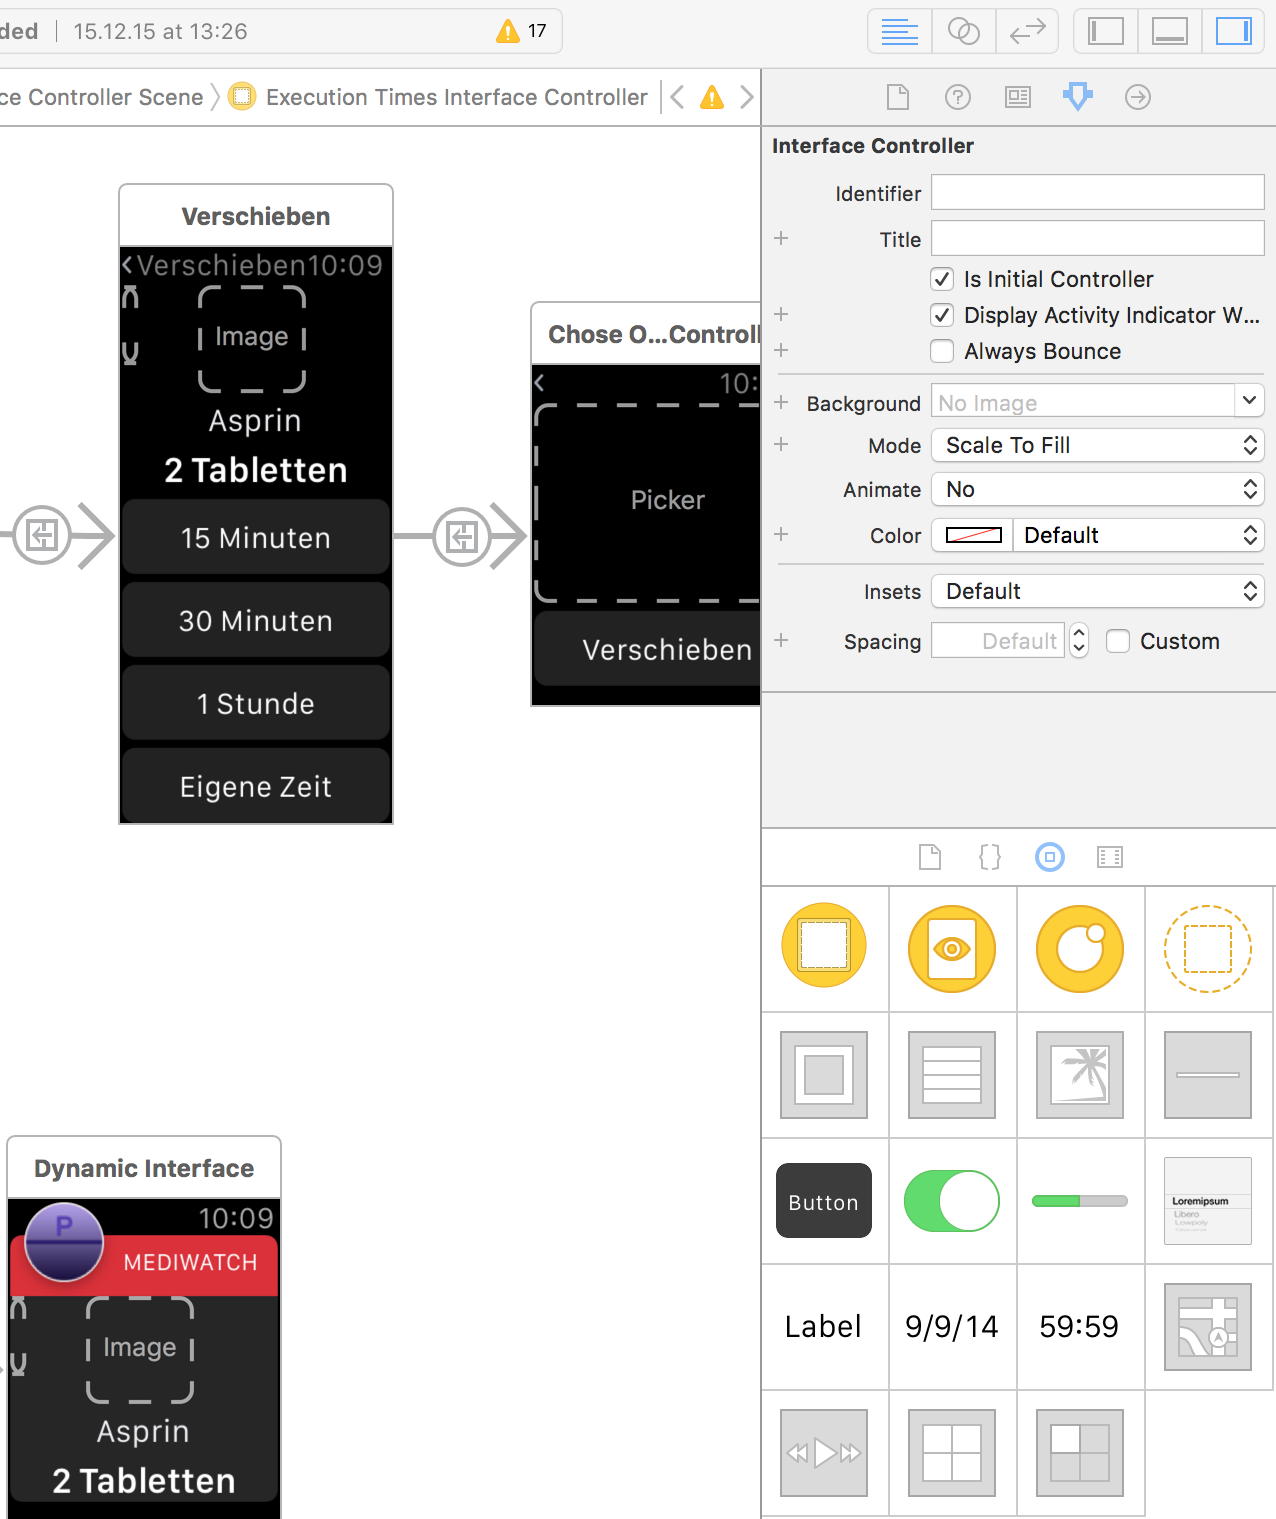
\includegraphics[width=0.9\textwidth]{04_realisation/screenshots/xcode-interface-elements}
\end{figure}

\begin{figure}
	\caption{Interface Elemente mit Quellcode verknüfen}
	\label{fig:xcode-interface-code-connect}
	\centering
	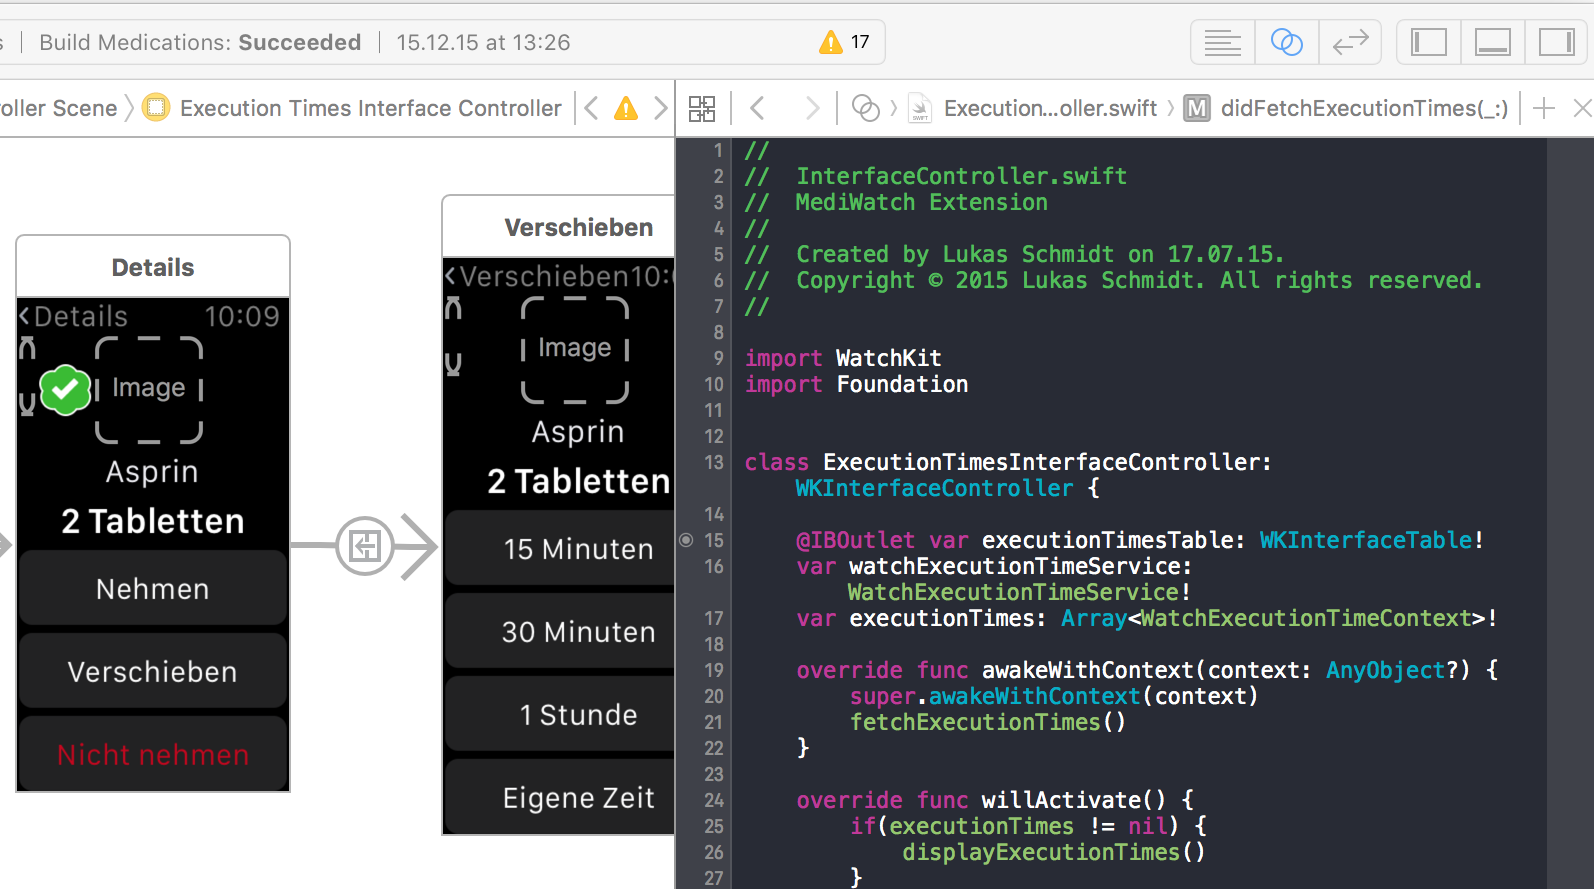
\includegraphics[width=0.9\textwidth]{04_realisation/screenshots/xcode-interface-code-connect}
\end{figure}

\section{Datenhalten - Persistence}
Da das generell iPhone das primäre Objekt der Nutzung ist, bietet sich die Datenhaltung auf dem iPhone an. Apple bietet mit mit CoreData \cite{Apple:2015swiftOpen} eine Framework zur Persistierung von Object-Graphen. Dieses Framework bietet eine gute Abstraction und ist deswegen leicht zu integrieren. So bringt CoreData einen graphischen Editor mit, der es erlaubt Datenschemata schnell und einfach zu erstellen. Daten, die in CoreData gespeichter wurden, lassen sich mittel gezielten Datenbankanfragen abfragen. So muss keine eigene Logik zum Suchen und Sortieren implementiert werden. Auch bietet Schnittstellen zum Verwalten von Änderung in den Daten, so lassen sich schnell komplexe Anwendungen erstellen. Durch langjähriges Bestehen des CoreData Frameworks lässt sich eine stabile Nutzung garantieren.  CoreData lässt sich auch auf der AppleWatch nutzen. Dupliziert man nun die Datenhaltung vom iPhone auf die Uhr, müssen diese beiden Datensätze immer konsistent gehalten werden. Dieser Abgleich bei Änderung einer Datenhaltung ist aufwendig zu implementieren. Wir der Abgleich jedoch realisiert wird die Uhr nochmal ein Stück unabhängiger. 

Im konkreten Fall wurde keine doppelte Datenhaltung genutzt. Das iPhone ist also die zentrale Datenquelle. Die Apple Watch kann als Client betrachtet werden, der die Daten des iPhones präsentiert. Zur Realisierung eines Client-Server Verbindung zwischen Uhr und iPhone wurde das WatchConnectivity Framework genutzt welches in \ref{watchCon} beschreiben wird. Daten müssen vor dem Versenden an die Uhr jedoch immer in ein serialisierbares Format übertragen werden. Es können CoreData Objekte nicht direkt übertragen werden.


\section{WatchConnectivity}
\label{watchCon}
Wichtig für die Kommunikation zwischen Uhr und iPhone ist das WatchConnectivity Framework \cite{Apple:2015SharingDataToWatch}. Hierbei ist im Listing \ref{lst:wcConnect} zu sehen, wie genau eine Verbindung aufgebaut werden kann. Es wird auch demonstriert wie ein Datenaustausch realisiert werden kann. Wichtig ist, dass diese Verbindung zum richtigen Zeitpunkt im Application-Lifecycle aufgebaut wird, da es sonst zu Datenverlusten kommen kann.

\lstinputlisting[caption=Nutzung des WatchConnectivity Framework, label=lst:wcConnect]{04_realisation/code/WatchExecutionTimeService.swift}
 

Mit der \lstinline{sendMessage:} Methode können Nachrichten und Datenpakete gesendet werden, welche sich durch eine ID identifizieren lassen. Eine direkte Antwort auf eine solche Nachricht ist mittels eines Replay-Handlers möglich. So kann eine Art Request/Response Datentransfer realisiert werden. Zu beachten ist jedoch, dass die Kommunikation relativ langsam ist. Sie sollte nur verwendet werden um kleine Informationen zu senden.

Werden erst beim Watch-App Start benötigte Daten vom iPhone angefordert, kann dies zu einer großen Verzögerung führen. Daher sollten Informationen, die auf der Uhr angezeigt werden, nicht erst zum Zeitpunkt der Darstellung angefordert werden. Gibt es eine Datenänderung auf dem iPhone, die relevante Daten für die Uhr enthält, so sollten diese mit der Methode \lstinline{transferUserInfo:}  an die Uhr gesendet werden. Mit dem Aufrufen dieser Methode wird die übergebene Information nicht direkt zur Uhr geschickt. Das System sendet die Daten zu einem optimalen Zeitpunkt (starke Verbindung zur Uhr, mögliche WLAN Verbindung) an die Uhr. Wenn nun die Watch-App startet sind die Daten bereit und können direkt dargestellt werden.

Zum Übertragen von größeren Daten steht die Methode \lstinline{transferFile:} zur Verfügung. Die Methode verhält sich equivalent zu \lstinline{transferUserInfo:}, wird jedoch in der Realisierung nicht verwendet.

\section{Modellierung des Programmablaufes}
Apple empfiehlt für iOS und auch watchOS die Nutzung von \gls{mvc} als Grundlage zur Entwicklung. So existiert in watchOS die Klasse \lstinline{WKInterfaceController} als Supertyp für jeden ViewController. Jeder ViewController ist standardmäßig für einen Bildschirm zuständig. So wird hier als Beispiel in \ref{lst:viewController}  der Controller zur Darstellung von Medikamentendetails beschreiben.

Die mit \lstinline{IBOutlet} annotierten Variablen sind Referenzen für View Elemenet. So hält \lstinline{drugNameLabel} ein Label zur Darstellung des Medikamentennamens. Methoden die mit \lstinline{IBAction} sind Aktionen, die beim interagieren mit dem Interface ausgelöst werden. \lstinline{onTakeMedication} wird ausgelöst wenn der Nutzer den Button zum Bestätigung der Einnahme klickt. Der Prefix \lstinline{IB} steht bei den Annotationen für InterfaceBuilder, welcher zum Erstellen der View-Elemente genutzt wird (\ref{ch:userinterface}).

Zum Wechseln zwischen ViewControllern, also z.B. von der Darstellung einer Liste zu einer Detailansicht, führt Apple den Begriff Segue ein. Sein Segue beschreibt eine Übergang zwischen zwei ViewControllern. Es gibt zwei Typen von Segues: Push und Modal. Ein modaler Segue fährt vom untere Rand des Bildschirms über den vorherigen ViewController. Diese Interaktion fordert den Nutzer auf eine Eingabe oder Interaktion zu Tätigen. Ist diese Interaktion erfolgt verschwindet der ViewController wieder nach unten. Der Push Segue eignet sich dazu um mehrdimensionale Interaktionen zu gestalten. Information im Detail anzuzeigen ist eine Ideale Anwendung dafür. Der Segue fährt von der rechten Seite auf den aktuellen ViewController. Diese Interaktion vermittelt dem Nutzer eine Kontinuität. So kann dieser Segue sehr gut hintereinander genutzt wurden um immer tiefer in eine Informationstruktur vorzudringen. Der Segue lässt sich durch einen Button am oberen linken Rand wieder verlassen. Auch eine Wischgeste, die dem Nutzer erlaubt den ViewController wegzuschieben ist vorhanden. Der Push Segue ist den meisten Nutzer auch von iOS bekannt.

Durch die geringe Anzahl an Segues kann eine sehr konsistente Interaktion auf der ganzen Platform garantiert werden. Dies erleichtert dem Nutzer die Navigation.

Die überschriebene Methode \lstinline{awakeWithContext:} ist eine Lifecycle Methode des ViewControllers. Sie hilft Daten von einem ViewController zum nächsten zu geben. Die Daten werden vom vorhergehenden ViewController bereit gestellt. Dieser überschreibt die Methode \lstinline{contextForSegueWithIdentifier:} und kann nun Daten abhängig vom Identifier übergeben. So sind diese zwei Methode der einzige Kontaktpunkt von ViewController. Dies erhöht extrem die Kapselung der Komponenten.

\lstinputlisting[caption=ViewController zu Darstellen von Medikamentendetails, label=lst:viewController]{04_realisation/code/MedicationDetailsController.swift}

\section{Picker - Auswahl}
Mit \lstinline{WKInterfacePicker} bietet Apple ein Standard View-Componente zum Auswählen von Elementen aus einer Liste. Der Nutzer kann so mit der Digital-Crown die Elemente auswählen. Diese leicht zu integrierende Auswahl ist leicht zu bedienen und habt das Nutzungserlebnis von anderen Uhren ab.

\section{Notification Management}
Notifications für die Medikationen werden mit der Notification API  registriert \cite{Apple:2015notif}. Auch kann das Verhalten der Notifications angepasst werden. So können vordefinierte Aktionen wie \glqq Einnehmen\grqq  oder \glqq Verschieben\grqq in die Notifications konfiguriert werden.

Bei der Notification handelt es sich um eine UILocalNotification \cite{Apple:2015notif}. Die Art von Notification benötigt keinen \gls{remoteServer}, sondern wird vom verbundenen iPhone verwaltet. Zum jetzigen Zeitpunkt ist es nicht möglich UILocalNotification von der Uhr zu erstellen. Dies würde die Uhr im Falle der Mediwatch-Anwendung noch unabhängiger machen. Sind die Notifications einmal auf dem iPhone registriert, werden sie zum Ausführungszeitpunkt auf der Uhr angezeigt. Dazu ist keine Verbindung zum iPhone mehr nötig.

\section{Anwendung}

Die Anwendung besteht aus zwei Komponenten auf der Apple Watch. Eine native Notification  und eine auf der Uhr installierte und ausgeführte Anwendung (siehe \ref{ch:watch_software}). In \ref{fig:watch-real} finden sich Bilder der Anwendung auf der Uhr. Dies sind Screenshots, die mit Hilfe einer Bildbearbeitungssoftware eingefügt wurden. Diese Bilder können ein Gefühl für die echte Anwendung auf der Uhr vermitteln.

\subsection{Notification}
 Die Notification bringt die Uhr zum Zeitpunkt der geplanten Medikamenteneinnahme zum Vibrieren und lässt optional einen Ton erklingen. Dies führt dazu, dass der Anwender auf die Uhr blickt und an die bevorstehende Medikamenteneinnahme erinnert wird. Die Notification wurde daraufhin optimiert, sodass eine große graphische Repräsentation des Medikaments angezeigt wird. Dem Nutzer wird so die Wiedererkennung des Medikaments erleichtert (siehe \ref{fig:watch-app-notification}). Neben dem Medikamentennamen wird auch die Dosierung des Medikaments dargestellt. Mit nur einer Aktion wird dem Nutzer ermöglicht, die Medikamenteneinnahme zu bestätigen oder sie zu verschieben. Die Notification ist darauf ausgelegt eine sehr schnelle Interaktion zu ermöglichen, damit der Nutzer nicht länger als 10 Sekunden mit der Uhr interagieren muss (siehe \ref{fig:watch-app-notification}). Diese Zeit führt sich auf die Studie \glqq Smartwatch in vivo\glqq \cite{Pizza:2016} zurück.
 
 Diese Erweiterung der Notification mit dem Bild des Medikaments wird jedoch vom System geregelt. Dauert das rendern der Notification zu lange, stellt das System eine reine Textdarstellung der Notification dar. Dies führt zu einem gewaltigen Informationsverlust. Als Anwendungsentwickler hat man nur die Option seine Notification mit bestmöglicher Geschwindigkeit zu rendern um eine Textdarstellung zu vermeiden. Dies bietet jedoch keine Garantie für eine erweiterte Darstellung der Notification.
\begin{figure}
	\caption{Notification für ein Medikament}
	\label{fig:watch-app-notification}
	\centering
	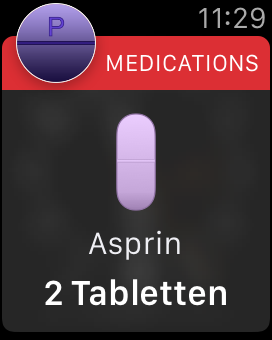
\includegraphics[width=0.4\textwidth]{04_realisation/screenshots/watch/notification01.png}
	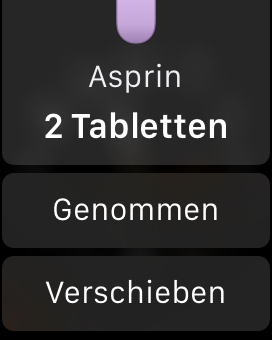
\includegraphics[width=0.4\textwidth]{04_realisation/screenshots/watch/notification02.png}
\end{figure}

\subsection{Native Anwendung}
Neben der Notification gibt es noch eine native App. Diese läuft auf der Uhr und stellt eine Liste der Medikamente des aktuellen Tages dar. Die App muss aktiv vom Nutzer gestartet werden. Der Nutzer muss also auf die Digital Crown drücken und dann die App aus der Übersicht wählen. In Abbildung \ref{fig:watch-app-take} wird ein Medikament aus der Liste ausgewählt. Nachdem man ein Medikament ausgewählt hat, bekommt man in einer Detailansicht das Medikament zu sehen. Nun kann das Medikament als genommen oder nicht genommen markiert werden. Ein visuelles Feedback (grüner Haken) zur Einnahme zeigt dem Nutzer seine Aktionen an. Von der Detailansicht aus ist es auch möglich, ein Medikament zur späteren Einnahme zu markieren. Hier hat der Anwender die Wahl aus vordefinierten Zeiten auszuwählen oder eine eigene Zeit zu bestimmen. Um die gewählte Zeitdauer wird die Benachrichtigung für das Medikament verschoben (siehe \ref{fig:watch-app-delay}). 

\begin{figure}
	\caption{Native Anwendung: Interface zum Wählen eines Medikaments (oben links). Medikament als genommen bestätigen (oben rechts). Eigene Zeitdauer auswählen (unten links). Medikament ist in der Übersicht als verschoben markiert (unten rechts)}
	\label{fig:watch-app-take}
	\centering
	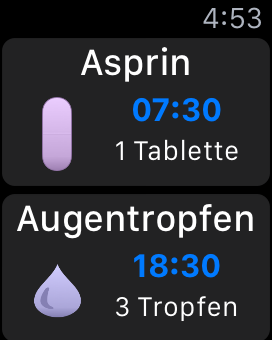
\includegraphics[width=0.4\textwidth]{04_realisation/screenshots/watch/notTaken01.png}
	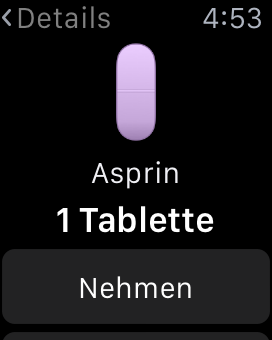
\includegraphics[width=0.4\textwidth]{04_realisation/screenshots/watch/notTaken02.png}
	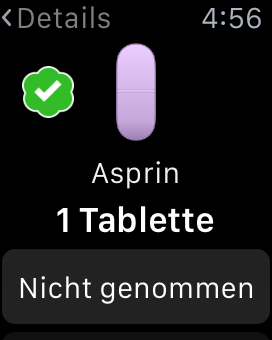
\includegraphics[width=0.4\textwidth]{04_realisation/screenshots/watch/taken01.png}
	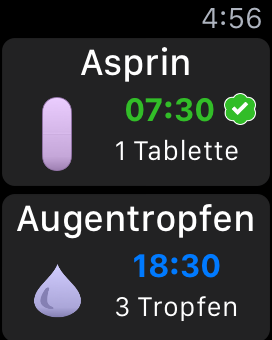
\includegraphics[width=0.4\textwidth]{04_realisation/screenshots/watch/taken02.png}
\end{figure}

\begin{figure}
	\caption{Native Anwendung: Interface zum Verschieben eines Medikaments (oben links). Zeitdauer für das Verschieben wählen (oben rechts). Medikament ist als genommen markiert (unten links). Medikament ist in der Übersicht als genommen markiert(unten rechts)}
	\label{fig:watch-app-delay}
	\centering
	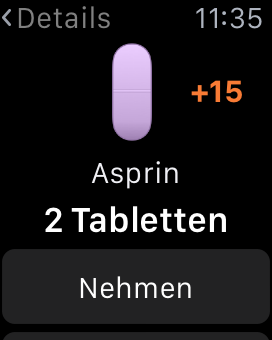
\includegraphics[width=0.4\textwidth]{04_realisation/screenshots/watch/delay01.png}
	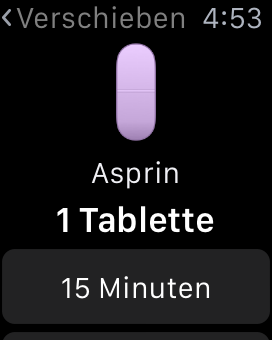
\includegraphics[width=0.4\textwidth]{04_realisation/screenshots/watch/delay02.png}
	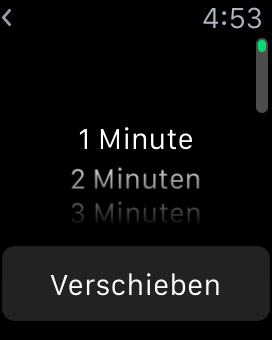
\includegraphics[width=0.4\textwidth]{04_realisation/screenshots/watch/delay03.png}
	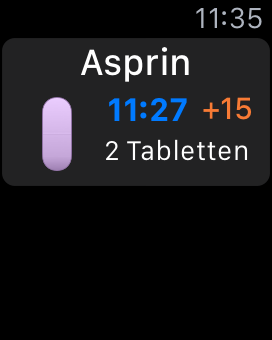
\includegraphics[width=0.4\textwidth]{04_realisation/screenshots/watch/delay04.png}
\end{figure}


\begin{figure}
	\caption{Native Anwendung - Dargestellt auf realen Uhren}
	\label{fig:watch-real}
	\centering
	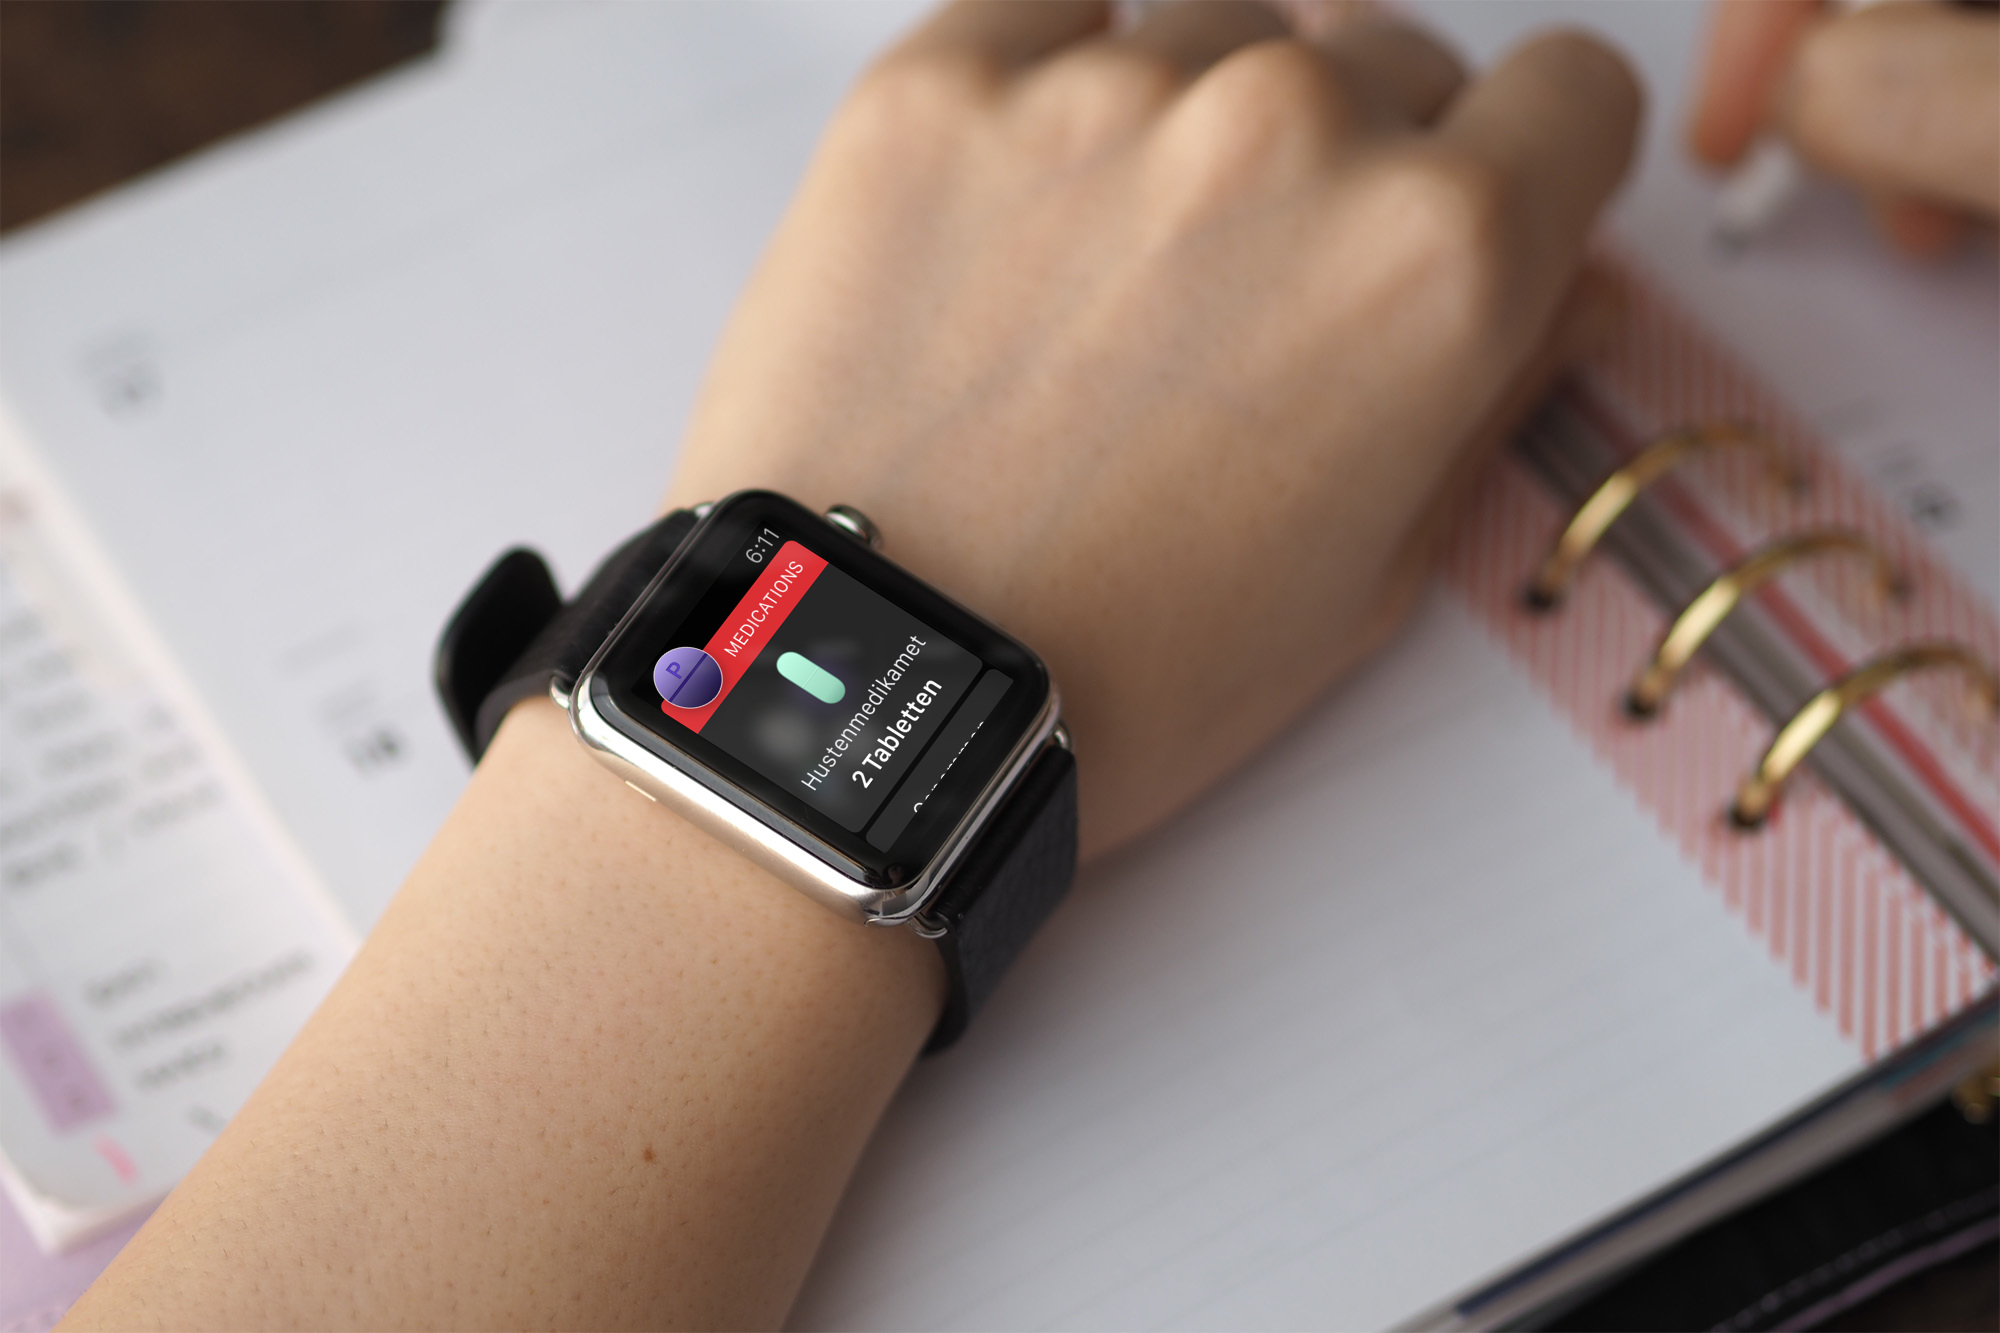
\includegraphics[width=1\textwidth]{04_realisation/screenshots/Mockup-Generated-by-Dunnnk.jpg}
	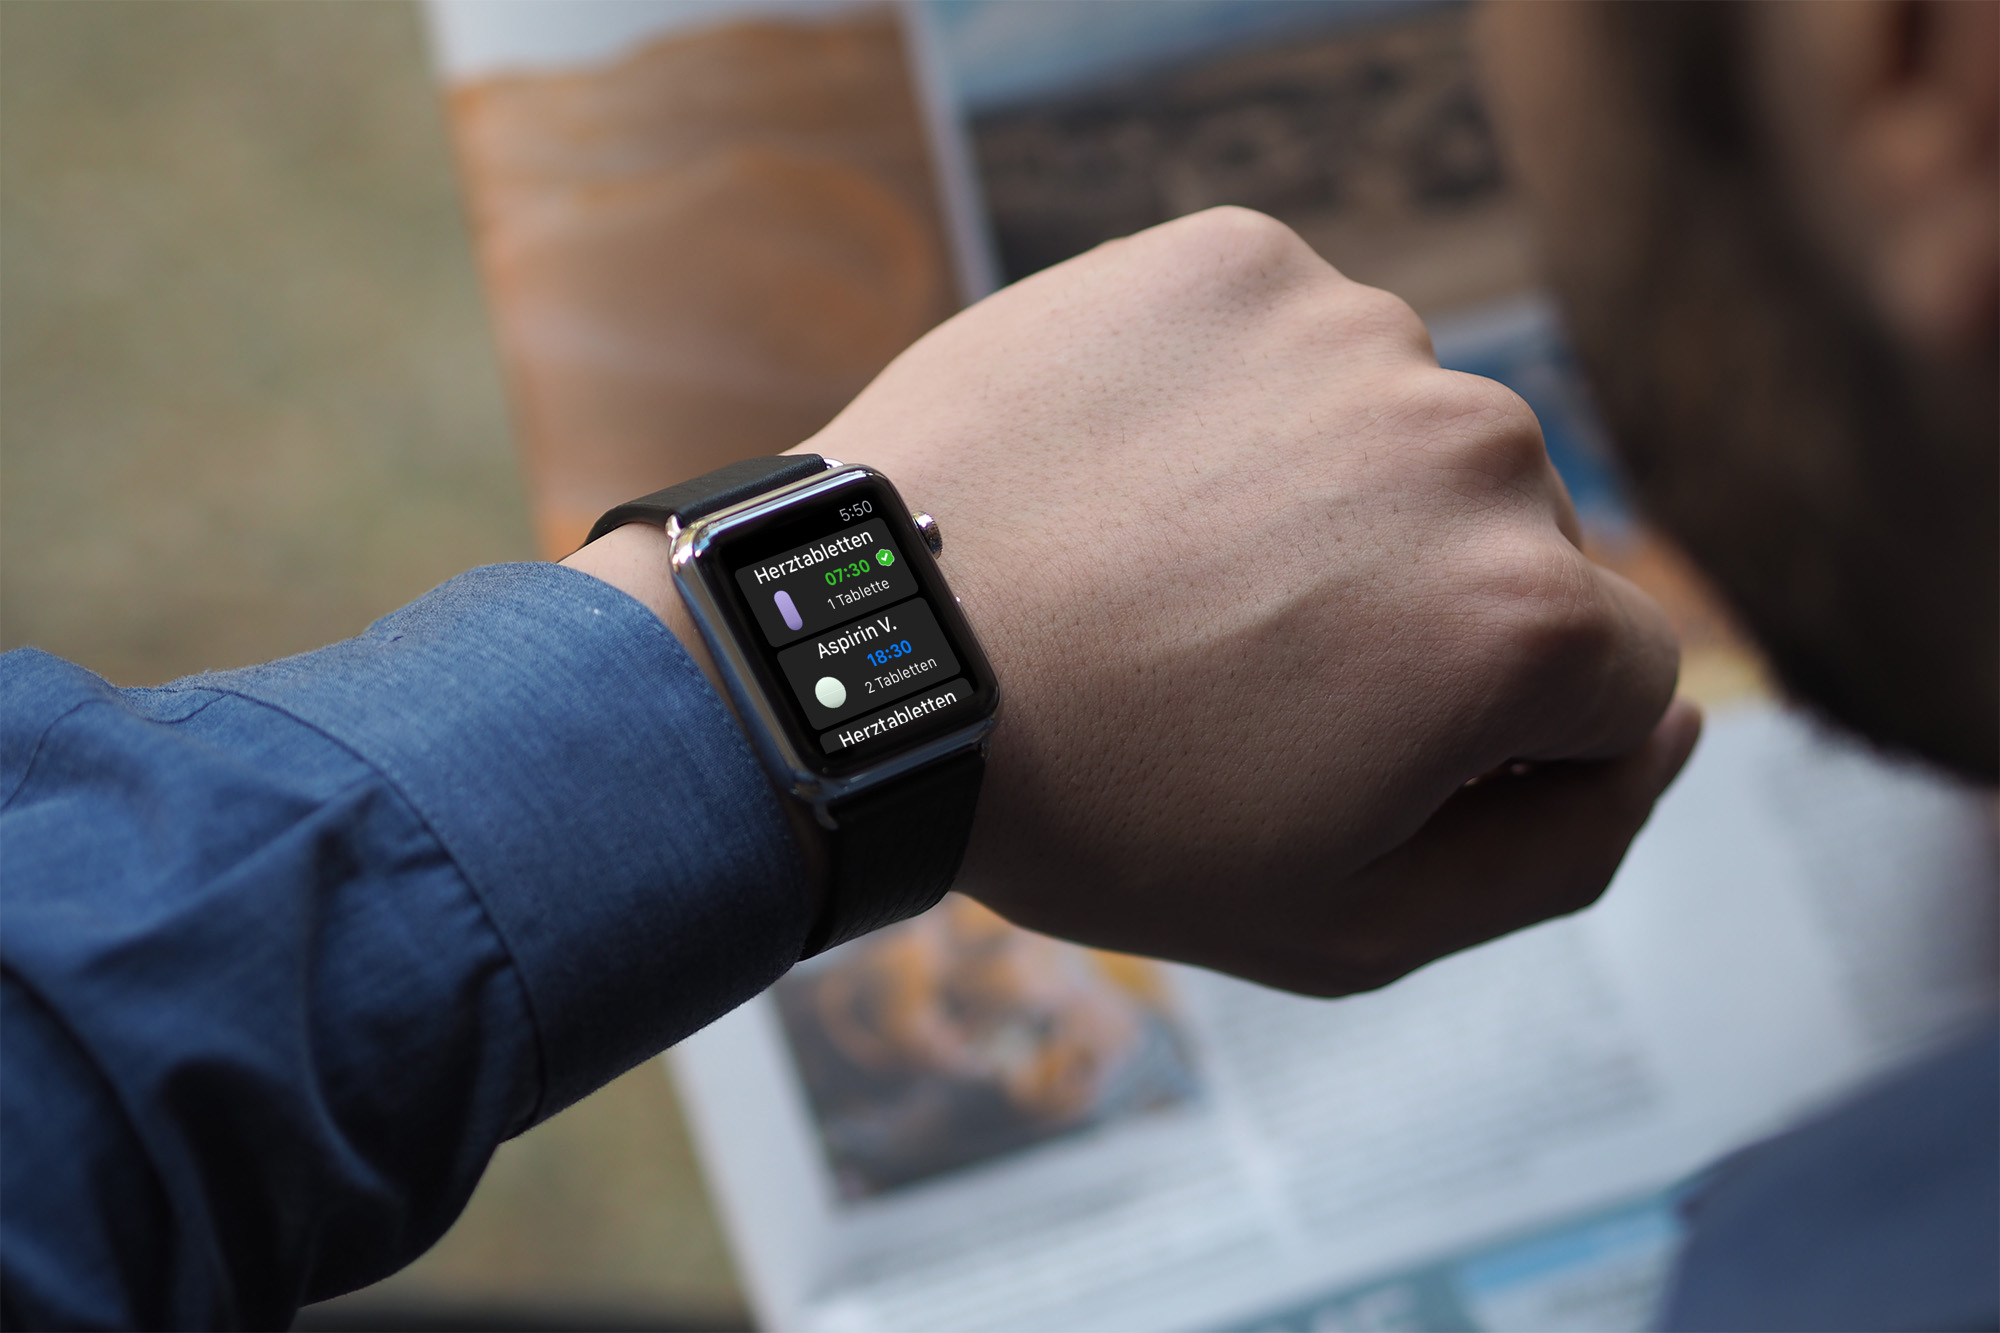
\includegraphics[width=1\textwidth]{04_realisation/screenshots/Mockup-Generated-by-Dunnnk-2.jpg}
	\end{figure}
\section{Quellcode}
Das ausführbare Projekt lässt sich von Github unter folgender URL\cite{Schmidt:repoCode} auschecken. So kann es kompiliert und getestet werden. 


 	
\chapter{Zusammenfassung, Evaluation und Ausblick}
\label{ch:summ-eva-outl}
 	%%
% ----------------------------------------------------------------------------
% "THE BEER-WARE LICENSE" (Revision 42):
% <sebastian.rauh@hs-heilbronn.de/michael.bauer@hs-heilbronn.de> wrote this 
% file. As long as you retain this notice you can do whatever you want with 
% this stuff. If we meet some day, and you think this stuff is worth it, you 
% can buy us a beer in return. 
% Michael Lukas Bauer, Sebastian Felix Rauh
% ----------------------------------------------------------------------------
%%

\section{Evaluation}

Die Evaluierung des Prototypen soll eine quantifiziertes Ergebnis liefern, anhand dessen Schwachstellen aufgezeigt werden sollen. Diese Schwachstellen sollen mit der nächsten Interation der Software ausgebessert werden.

\subsection{Zielgruppe}
Die Zielgruppe sollten Menschen sein, deren Alltag von Medikamenteneinnahmen geprägt ist. Es sollte sich um Menschen mit wenig oder keinen Vorkenntnissen mit Touchscreen-basierten Geräten handeln.  Patienten fortgeschrittenen Altern, die sich stationär im Krankenhaus aufhalten eignen sich gut, Medikamente nehmen und viel freie Zeit während des Aufenthaltes im Krankenhaus für eine Befragung haben.

\subsection{Vorgehen}
Im ersten Schritt wird der Zielgruppe die Apple Watch gezeigt und die dahinterliegende Technologie erklärt, um Neugier bei den Patienten zu wecken. Nun können die Patienten die Uhr anlegen. 
Im zweiten Schritt wird ein Notification, die eine Vibration auslöst gestartet. Die Patienten müssen die Vibration spüren und dann auf die Uhr schauen. Dort sollen sie den Bildschirminhalt wiedergeben. Haben sie den Bildschirminhalt wiedergegeben, so müssen sie die Benachrichtigung bestätigen, also auf den Button mit der Aufschrift "Genommen" tippen.

In Schritt Drei müssen die Patienten durch drücken auf die digital Crown den App Bildschirm aufrufen um dort die Mediwatch App zu öffnen. Wenn die App geöffnet ist, soll ein Medikament ausgewählt werden und dieses um eine definierte Zeit verschoben werden. Ist das Medikament verschoben, so ist die Aktion beendet.

\subsection{Auswertung}
Für die Evaluation werden 2 Fragebögen genutzt. Einmal AttrakDiff\cite{UserInDe:Attrakdiff}, welcher die subjektiv  Wahrnehmung der Bedienbarkeit und Aussehen des Prototypen erfragt. Es handelt sich um einen standardisierten Fragebogen und eine standardisierten Auswertungsmethode. Da dieser Frageboden keine Antworten über Funktionen des Prototyp gibt, ist es nötig einen zweiten Fragebogen zu erstellen. Dieser Fragebogen erfragt die Situation, also den Kontext in dem sich der Anwender befindet und die daraus Folgenden Ansprüche an den Prototypen. So sollen fehlende Funktionen oder Fehler in der Analyse aufdecken werde. Die Fragen sind im Anhang zu finden.
Die Erfassung der Fragen wird mit Limesurvey\cite{Limesurvey} in Version 2.05 durchgeführt. Da sich Limesurvey selbst hosten lässt, bleiben die erfragten Daten auf einem sicheren Hochschulserver und werden nicht bei Drittanbietern gespeichert. 

\section{Durchführung der Evaluation}
\subsection{Beschreibung der Zielgruppe}
Es haben insgesamt 11 Patienten  an der Befragung teilgenommen. Davon waren 7 weiblich und 4 männlich. Alle waren im Alten zwischen 70 und 85. 

\subsection{Befragung der Patienten}
Die Befragung in der Zielgruppe verlief sehr schwierig und nicht wie geplant.
Der erste Schritt der Befragung klappte bei fast allen Probanden sehr gut. So erkannten alle die Notification mit der einhergehenden Vibration wurde von allen Patienten als verständlich geschildert. Das darauf folgende Bestätigen einer Notification verlief zu großen Teilen schlecht. Die Patienten konnten die Buttons zum Bestätigen nicht treffen, da ihnen die Feinmotorik fehlte.
Öffnen einer App ist auf Grund der fehlenden Feinmotorik ebenfalls nicht möglich. Die App-Icons sind zu klein und werden nicht getroffen. Das öffnen der Anwendung wurde bei allen Patienten nicht erreicht.
\subsection{Auswertung}
Der Fragebogen AttrakDiff ist in dieser Zielgruppe nicht praktikabel. Eine sehr genauer Unterscheidung zwischen den Begrifflichkeit, die der  AttrakDiff abfragt ist für die Zielgruppe nicht möglich. Dies fällt auf, wenn man mit den Probanden spricht. Die Probanden schweifen oft ab und es ist nicht möglich ihre Aussagen zu erfassen. Direkte Fragen, die den Alltag der Probanden betreffen werden zuverlässig beantwortet. Schwierigkeiten, die bei der Medikamenten Einnahme werden nicht zugegeben.
Die Befragung wurden deswegen auf eine Thinking Alound Methode \cite{Sommerville:2016aa} umgestellt. Leider sind die Ergebnisse so nicht mehr quantifizierter, jedoch sind aus des Aussagen der Patienten und den Beobachtungen gute Schlussfolgerungen möglich.
Auch der der zweite Fragebogen zu den Funktionen und deren Nutzungskontext wurde nicht genutzt. Hier wurde versucht 
Während er Gesprächs  mehr Einblick in das Leben der Probanden zu erhalten. Probanden erzählen gerne über ihr Leben und suchen eher das persönliche Gespräch. Aus diesen Gesprächen geht hervor, dass die Patienten mit großer Übereinstimmung keinen Internetanachluss besitzen. Dies schließt entfernte Aktualisierungen des Mediktionsplans und Einnahme Bestätigungen für den Arzt aus. Bedenken äußern die Weiblichen Patientinnen über die Größe und das Aussehen der Uhr. Eine Uhr muss dem Geschmack der Patientin gefallen. Hierbei spielt die Größe der Uhr, wie auch das Aussehen eine Rolle. Bei Beschreibung von anderen modischen Farben der Uhr oder der Armbänder, zeigen sie sich interessiert.  Ein Großteil der Patienten sieht jedoch ein, dass sie auf Grund Ihrer Sehschwäche die große Uhr (42mm) brauchen. Die große Uhr wird in Gegenzug als zu Groß beschrieben. Die meisten Patienten haben keine Probleme die Schrift zu lesen. Meist nehmen Sie Ihre Brille zur Hilfe, die im Krankenhaus natürlich immer griffbereit ist. Nur bei einem kleine Teil kommt es vor, dass sie den Text auf dem Display auch mit Brille nicht lesen können. Das größte Problem ist jedoch die schon genannte fehlende Feinmotorik. So können die Probanden die Uhr nicht wirklich aktiv bedienen, sondern reagieren nur auf die Vibration am Handgelenk. Dies führt zu einer Hilflosigkeit gegenüber der Technik der Uhr.
\subsection{Probleme tabellarisch}
\begin{table}[]
\centering
\caption{Probleme und mögliche Lösungen des Smartwatch Prototypes}
\label{my-label}
\begin{tabular}{p{4cm} p{5cm} p{5cm}|l|l|l|}
\hline
 Problem  &Auswirkungen  &mögliche Lösung  \\ \hline
 \textbf{fehlender Internetanschluss}  &keine Aktualisierungen des Medikamentenplans und keine Benachrichtigungen für den Arzt &Uhr oder Smartphone mit Mobilfunkverbindung ausstatten  \\
 \textbf{fehlende Feinmotorik der Probanden} &Buttons werden nicht getroffen oder falsche Aktionen werden ausgelöst  &große haptische Knöpfe in die Hardware integrieren, die gut drückbar sind  \\
 \textbf{Vibration zu leicht}&Vibration wird nicht gespürt und Medikament wird vergessen  &Stärkere Vibration,Lauten Ton dazu abspielen, starken optisches Feedback (grelles Blinken)   \\
 \textbf{Nur mit Brille lesbar} &Benachrichtigung wird erkannt, bis jedoch die Brille im Haushalt gefunden, ist die Medikation schon vergessen oder die Uhr hat die Benachrichtigung schon zurückgestellt  &Größeres Schrift, die Auch ohne Brille lesbar ist. Audiowiedergabe der Medikation  \\
 \textbf{Armband schwer anlegbar}&Uhr wird morgens nicht gerne Angezogen und bleibt so liegen und Patient bekommt keine Benachrichtigungen  &Verzicht auf Standart Sport Band und dafür Armbänder die leicht anzuziehen sind finden. Viele Patienten tragen dehnbare Bänder ohne Verschluss \\
 \textbf{Uhr ist unästhetisch}&Patient trägt die Uhr nicht und wird so nicht an die Medikamente erinnert  &Keine Standart Uhren kaufen, sondern den Patienten die Farbe und Form der Uhr und die Art des Armbandes aussuchen lassen  \\ \hline
\end{tabular}
\end{table}

\section{Zusammenfassung}
Ziel der Arbeit war es, die Akzeptanz eines Systems zur Erinnerung an Medikamente zu testen. Dieses Ziel wurde mit einer Patientenbefragung verfolgt. Patienten stehen dem Konzept der Uhr am Handgelenk, ob sie jetzt digital oder Analog ist positiv gegenüber. So ist die Uhr als Medium für solche Zwecke geeignet. Die Apple Watch, mit ihrer touchscreenbasierten Navigation, stellt für die getestete Zielgruppe eine große Herausforderung da. Fehlende Feinmotorische Fähigkeiten erschwert den Patienten die Interaktion mit der Uhr. Auch sind Vibration und Geräuschwiedergabe zu schwach und können so leicht überhört werden. Das ästhetische Aussehen der Uhr ist nicht zu vernachlässigen, da die Uhr oft als Art Schmuck getragen wird. So trägt die Farbe, Form und Größe zur Akzeptanz der Uhr bei. Findet der Patient die Uhr unschön/unmodisch, so wird er sie nicht tragen und schlimmstenfalls seine Medikamente vergessen.

Da Smartwatches noch keine große Verbreitung haben, sind auch die Werkzeuge zur Umsetzung von Anwendungen begrenzt. Interaktive Prototypen sind auf der Uhr nicht die Verwendung von Code möglich. So vermehrt sich der Aufwand für schnelles iteratives Vorgehen. Das WatchOS SDK von Apple bietet eine relativ übersichtliche Schnittstelle. Die Schnittstellen ermöglichen es komplexere Anwendungen zu erstellen. Diese sind jedoch an manchen Stellen noch limitiert. Da es sich um die erste Geräte-Generation handelt, muss abgewartet werden, mit welchen Leistungsverbesserungen weiter Generation nachgerüstete werden, um die Uhr zu einem wirklich nützlichen Werkzeug zu machen. Das Potential zu einem guten Nutzen zeigt die erste Generation auf, jedoch ist sie an manchen Stellen (Geschwindigkeit, Lange Wartezeiten) noch nicht ausgereift.

Apples neue Programmiersprache Swift, die zur Implementierung genutzt wurde, bietet Konzepte moderner Programmiersprachen. Diese Konzepte unterstützen den Entwickler meist schon zur Compilezeit. Dies führt zu einer frühen Fehlererkennung. Durch diese Spracheigenschaften, wie Optionals (\ref{ch:optionals}), die Sicherheit in der Modelierung geben oder Closures und First Class Functions (\ref{ch:closures}) die Konzepte Funktionales Programmierung bereitstellen, eignet sich Swift sehr gut als Lehrsprache. Dadurch das Swift unter einer Open Source Lizenz veröffentlicht wurde, kann man nun für mehre Zielplattfomen Entwickeln.

\section{Ausblicke}
Mit den Gewonnen Ergebnissen kann diese Projekt neu ausgerichtet werden. So sollte die Zielgruppe über mehr Erfahrung mit digitalen Geräten verfügen. So wäre eine Unterstützung von Kindern und Jugendlichen im Alter ab 12 Jahren denkbar. Diese könnten bei ihrer Therapie unterstützt werden und durch die moderne Technik, mit der sie aufgewachsen sind, motiviert werden, Medikamente zeitgemäß einzunehmen.
Nachdem die Defizite mit der Lesbarkeit durch die Evaluation entdeckt wurden, ergab die Recherche, dass die watchOS Plattform über Funktionen der Accessibility verfügt \cite{Apple:watchAccess} . Damit ist es möglich Nutzungs-Erleichterungen für Menschen mit Körperlichen Einschränkungen zu schaffen. So kann mit DynamicType, also eine dynamischen Schriftgröße in der App, die Lesbarkeit verbessert werden. Der Nutzer kann so seine eigene Schriftgröße wählen. Auch die Navigation zum Öffnen von Anwendungen wird mit Accessibility Einstellungen verbessert.

\twocolumn 
\bibliography{06_appendix/03_bibliography/bib}

\onecolumn
\appendix 	
\chapter{Appendix}
\label{ch:appendix}
 	%
% ----------------------------------------------------------------------------
% "THE BEER-WARE LICENSE" (Revision 42):
% <sebastian.rauh@hs-heilbronn.de/michael.bauer@hs-heilbronn.de> wrote this 
% file. As long as you retain this notice you can do whatever you want with 
% this stuff. If we meet some day, and you think this stuff is worth it, you 
% can buy us a beer in return. 
% Michael Lukas Bauer, Sebastian Felix Rauh
% ----------------------------------------------------------------------------


\section{Fragebogen}
\begin{enumerate}
\item Tragen Sie eine Uhr im Alltag?
\begin{tasks}(4)
\task Ja
\task Nein
\end{tasks}
\item Wären Sie bereit eine digitale Computeruhr zu tragen?
\begin{tasks}(4)
\task Ja
\task Nein
\end{tasks}
\item Finden Sie die Idee gut, von der Uhr an Ihre Medikamenteneinnahme erinnert zu werden?
\begin{tasks}(4)
\task Ja
\task Nein
\end{tasks}
\item Finden Sie die Idee gut, von der Uhr an ihre genauen Medikamente erinnert zu werden?
\begin{tasks}(4)
\task Ja
\task Nein
\end{tasks}
\item Wie viele Medikamente nehmen Sie täglich?
\begin{tasks}(4)
\task Ein Medikament
\task Mehr als drei
\task Mehr als fünf
\task Mehr als acht
\end{tasks}
\item Haben Sie Probleme, Ihre Medikamente rechtzeitig zu nehmen?
\begin{tasks}(4)
\task Ja
\task Nein
\end{tasks}
\item Wissen Sie welche Medikamente Sie nehmen?
\begin{tasks}(4)
\task Ja
\task Nein
\end{tasks}
\item Können Sie die Medikamente an Form und Farbe unterscheiden?
\begin{tasks}(4)
\task Ja
\task Nein
\end{tasks}
\item Haben Sie einen Internetzugang zu Hause?
\begin{tasks}(4)
\task Ja
\task Nein
\end{tasks}
\item Benutzen Sie einen Computer?
\begin{tasks}(4)
\task Ja
\task Nein
\end{tasks}
\item Benutzen Sie ein mobiles Telefon?
\begin{tasks}(4)
\task Ja
\task Nein
\end{tasks}
\item Würden Sie die Erinnerung an die Medikamente mit der Uhr nutzen?
\begin{tasks}(4)
\task Ja
\task Nein
\end{tasks}
\item Welche Funktionen fehlen, die Sie als wichtig ersehen?
\item Gibt es Funktionen, die Sie für unwichtig halten?
\end{enumerate}
 
 		
\chapter{Dokumentation}
\label{ch:documentation}
 	%%
% ----------------------------------------------------------------------------
% "THE BEER-WARE LICENSE" (Revision 42):
% <sebastian.rauh@hs-heilbronn.de/michael.bauer@hs-heilbronn.de> wrote this 
% file. As long as you retain this notice you can do whatever you want with 
% this stuff. If we meet some day, and you think this stuff is worth it, you 
% can buy us a beer in return. 
% Michael Lukas Bauer, Sebastian Felix Rauh
% ----------------------------------------------------------------------------


\section{Fragebogen}
\begin{enumerate}
\item Tragen Sie eine Uhr im Alltag?
\begin{tasks}(4)
\task Ja
\task Nein
\end{tasks}
\item Wären Sie bereit eine digitale Computeruhr zu tragen?
\begin{tasks}(4)
\task Ja
\task Nein
\end{tasks}
\item Finden Sie die Idee gut, von der Uhr an Ihre Medikamenteneinnahme erinnert zu werden?
\begin{tasks}(4)
\task Ja
\task Nein
\end{tasks}
\item Finden Sie die Idee gut, von der Uhr an ihre genauen Medikamente erinnert zu werden?
\begin{tasks}(4)
\task Ja
\task Nein
\end{tasks}
\item Wie viele Medikamente nehmen Sie täglich?
\begin{tasks}(4)
\task Ein Medikament
\task Mehr als drei
\task Mehr als fünf
\task Mehr als acht
\end{tasks}
\item Haben Sie Probleme, Ihre Medikamente rechtzeitig zu nehmen?
\begin{tasks}(4)
\task Ja
\task Nein
\end{tasks}
\item Wissen Sie welche Medikamente Sie nehmen?
\begin{tasks}(4)
\task Ja
\task Nein
\end{tasks}
\item Können Sie die Medikamente an Form und Farbe unterscheiden?
\begin{tasks}(4)
\task Ja
\task Nein
\end{tasks}
\item Haben Sie einen Internetzugang zu Hause?
\begin{tasks}(4)
\task Ja
\task Nein
\end{tasks}
\item Benutzen Sie einen Computer?
\begin{tasks}(4)
\task Ja
\task Nein
\end{tasks}
\item Benutzen Sie ein mobiles Telefon?
\begin{tasks}(4)
\task Ja
\task Nein
\end{tasks}
\item Würden Sie die Erinnerung an die Medikamente mit der Uhr nutzen?
\begin{tasks}(4)
\task Ja
\task Nein
\end{tasks}
\item Welche Funktionen fehlen, die Sie als wichtig ersehen?
\item Gibt es Funktionen, die Sie für unwichtig halten?
\end{enumerate}
 
\end{document}
